\documentclass[11pt]{amsart}
\usepackage[utf8]{inputenc}
\usepackage[T1]{fontenc}
\DeclareUnicodeCharacter{1D9C}{\ensuremath{^{\mathsf{c}}}}
\usepackage{lmodern}
\usepackage[margin=1.1in]{geometry}
\usepackage{amsmath,amssymb,amsthm,mathtools}
\usepackage{enumitem}
\usepackage{booktabs,tabularx,longtable,array}
\usepackage{tikz}
\usetikzlibrary{arrows.meta,positioning,shapes.geometric,fit,calc,backgrounds,decorations.pathreplacing}
\usepackage{xcolor}
\usepackage{listings}
\usepackage{xurl}
\usepackage[colorlinks=true,linkcolor=blue!50!black,citecolor=green!40!black,urlcolor=blue!60!black]{hyperref}

\hypersetup{pdftitle={The Erdos-Hajnal property for the six-vertex path},pdfauthor={Claude (Anthropic)}}

\definecolor{nonedge}{RGB}{200,40,40}
\definecolor{edgegrey}{RGB}{150,150,150}
\definecolor{imported}{RGB}{255,236,200}
\definecolor{newpart}{RGB}{214,234,255}

% ---------------------------------------------------------------- Lean listings
\lstdefinelanguage{lean}{
  morekeywords={axiom,theorem,lemma,def,fun,Type,Prop,Finset,SimpleGraph,Fintype,DecidableEq,DecidableRel},
  sensitive=true, morecomment=[l]{--}, morestring=[b]"
}
\lstset{language=lean, basicstyle=\ttfamily\footnotesize, keywordstyle=\bfseries,
  columns=fullflexible, keepspaces=true, breaklines=true, frame=single, rulecolor=\color{black!25},
  xleftmargin=0.5em, xrightmargin=0.5em, aboveskip=0.6em, belowskip=0.6em,
  literate=
   {∀}{{$\forall$}}1 {∃}{{$\exists$}}1 {→}{{$\to$}}1 {∧}{{$\wedge$}}1 {∨}{{$\vee$}}1
   {¬}{{$\neg$}}1 {≤}{{$\le$}}1 {≠}{{$\ne$}}1 {⊆}{{$\subseteq$}}1 {∈}{{$\in$}}1
   {ℝ}{{$\mathbb{R}$}}1 {ℕ}{{$\mathbb{N}$}}1 {ᶜ}{{$^{\mathsf{c}}$}}1 {⌊}{{$\lfloor$}}1
   {⌋}{{$\rfloor$}}1 {₊}{{$_{+}$}}1 {↔}{{$\leftrightarrow$}}1 {Δ}{{$\Delta$}}1
   {ε}{{$\varepsilon$}}1 {δ}{{$\delta$}}1 {ℓ}{{$\ell$}}1 {β}{{$\beta$}}1 {τ}{{$\tau$}}1
}

% ---------------------------------------------------------------- theorems
\newtheorem{theorem}{Theorem}[section]
\newtheorem{lemma}[theorem]{Lemma}
\newtheorem{corollary}[theorem]{Corollary}
\newtheorem{proposition}[theorem]{Proposition}
\newtheorem{claim}{Claim}
\newtheorem{theoremL}{Theorem}
\renewcommand{\thetheoremL}{\Alph{theoremL}}
\newtheorem{importedthm}{Imported Theorem}
\renewcommand{\theimportedthm}{\Roman{importedthm}}
\newtheorem*{conjecture}{Conjecture (Erd\H{o}s--Hajnal)}
\theoremstyle{definition}
\newtheorem{definition}[theorem]{Definition}
\theoremstyle{remark}
\newtheorem{remark}[theorem]{Remark}

% ---------------------------------------------------------------- macros
\newcommand{\cP}{\overline{P_6}}
\newcommand{\Gbar}{\overline{G}}
\newcommand{\eps}{\varepsilon}
\newcommand{\lean}[1]{\texttt{#1}}
\newcommand{\cL}{\mathcal{L}}
\newcommand{\cA}{\mathcal{A}}
\newcommand{\cF}{\mathcal{F}}
\newcommand{\cG}{\mathcal{G}}
\newcommand{\famP}{\mathcal{P}}
\newcommand{\famQ}{\mathcal{Q}}
\newcommand{\floor}[1]{\lfloor #1\rfloor}
\newcommand{\ceil}[1]{\lceil #1\rceil}
\newcommand{\repo}{\url{https://github.com/machine-qed/erdos-hajnal-six-vertex-path}}

\title{The Erd\H{o}s--Hajnal property for the six-vertex path}
% the empty optional argument keeps the author out of the running heads
\author[]{Claude (Anthropic)}
\thanks{This paper, the proof it contains and the accompanying Lean formalization were produced by
an AI system in a research session commissioned by the owner of the repository \repo, who is
responsible for their release. It is not a publication of Anthropic, and Anthropic has not
reviewed it. The paper has not been refereed. Please report problems as issues in that repository. The paper is
released under CC BY 4.0.}
\date{September 2026}

\begin{document}

\begin{abstract}
We prove that there is $\tau>0$ such that every graph on $n$ vertices with no induced path on six vertices
has a clique or a stable set with at least $n^{\tau}$ vertices; that is, the six-vertex path $P_6$ has
the Erd\H{o}s--Hajnal property. The proof follows the proof of Nguyen, Scott and Seymour for the
five-vertex path and replaces the two steps of that proof which use the absence of an induced house. One
replacement is structural: a \emph{module law} forced by the absence of the complement of $P_6$, combined
with the modular decomposition of the teeth of a comb (the \emph{Tooth Lemma}), shows that combs can be
cleaned into blockades whose pairs are complete or sparse on average, and the layout theorem of Nguyen,
Scott and Seymour accepts such blockades. The other replacement shows that the blocks on which a vertex
is lightly mixed induce a house-free pattern, so that the Erd\H{o}s--Hajnal theorem for $P_5$ can be
applied to the pattern. The whole argument has been formalized in Lean~4 with Mathlib. The formalization
also proves one of the four cited theorems, takes the other three as hypotheses, and has been checked
both by Lean's kernel and by an independent type checker.
\end{abstract}

\maketitle
\setcounter{tocdepth}{1}
\tableofcontents

\section*{Introduction}

A graph $G$ is \emph{$H$-free} if no induced subgraph of $G$ is isomorphic to $H$. Write $\hom(G)$ for
the largest size of a clique or a stable set of $G$. Every graph on $n$ vertices has $\hom(G)\ge
\frac12\log_2 n$, and random graphs show that this is best possible up to the constant. In 1977 Erd\H{o}s
and Hajnal~\cite{EH77,EH} conjectured that excluding a single induced subgraph changes the picture completely.

\begin{conjecture}
For every graph $H$ there exists $c>0$ such that every $H$-free graph $G$ satisfies $\hom(G)\ge|G|^{c}$.
\end{conjecture}

A graph $H$ for which this holds is said to have the \emph{Erd\H{o}s--Hajnal property}. The property is
known for every graph with at most four vertices and is preserved by substitution~\cite{APS}. The bull
was settled by Chudnovsky and Safra~\cite{CS}, and the five-cycle by Chudnovsky, Scott, Seymour and
Spirkl~\cite{C5}. Nguyen, Scott and Seymour proved it for the five-vertex path~\cite{NSS7}, which settled
every graph on five vertices. Since then it has been proved for a few six-vertex graphs: the E-graph and
the bird~\cite{HJZ}, and the graph with edges $ab,bc,cd,de,af,bf,df$~\cite{TN}. For paths in general,
Nguyen, Scott and Seymour~\cite{NSS5} showed that $P_k$-free graphs satisfy $\hom(G)\ge
2^{(\log|G|)^{1-o(1)}}$, and Bousquet, Lagoutte and Thomass\'e~\cite{BLT} proved a polynomial bound when
both $P_k$ and its complement are excluded. After $P_5$, the six-vertex path $P_6$ is the smallest path
for which the conjecture was open.

\begin{theoremL}\label{thm:main}
There exists $\tau>0$ such that every $P_6$-free graph $G$ satisfies $\hom(G)\ge|G|^{\tau}$.
\end{theoremL}

A graph is $P_6$-free if and only if its complement is $\cP$-free, and $\hom(G)=\hom(\Gbar)$, so
Theorem~\ref{thm:main} is equivalent to the Erd\H{o}s--Hajnal property of $\cP$. We work with
$\cP$-free graphs throughout. We in fact prove the stronger \emph{polynomial R\"odl property}
(Theorem~\ref{thm:polyrodl}): there is $A$ such that for every $\eps\in(0,\frac12)$, every $\cP$-free
graph $G$ has an induced subgraph on at least $\eps^{3A}|G|$ vertices whose maximum degree, or whose
complement's maximum degree, is at most $\eps$ times its number of vertices.

The proof determines $\tau$ by a formula (Table~\ref{tab:constants}) in the constant $\delta$ of R\"odl's
theorem and the exponent of the Erd\H{o}s--Hajnal theorem for $P_5$. No numerical values of these are
available, so we cannot give $\tau$ numerically; the formula only shows that $\tau<10^{-15}$.

\subsection*{What is new and what is inherited}
The proof uses four results from the literature as black boxes: R\"odl's theorem, a blockade theorem of Nguyen,
Scott and Seymour for sparse graphs without a long induced path, the Erd\H{o}s--Hajnal theorem for
$P_5$, and the comb lemma of Chudnovsky, Scott, Seymour and Spirkl. The architecture of the proof
(iterative sparsification organised around combs, niceness and a layout theorem) is that of the proof for
$P_5$ by Nguyen, Scott and Seymour~\cite{NSS7}. That proof uses the absence of an induced \emph{house},
the complement of $P_5$, in exactly two places, and both fail for $\cP$-free graphs. The following parts
are new:
\begin{itemize}[leftmargin=1.5em]
\item the three six-vertex certificates: the module law (Lemma~\ref{lem:module}) and the diagonal and
  house lemmas (Lemmas~\ref{lem:diagonal} and~\ref{lem:house});
\item the Tooth Lemma (Lemma~\ref{lem:tooth}), which combines the module law with the modular
  decomposition of a comb's teeth;
\item the resulting comb lemma for $\cP$ (Lemma~\ref{lem:comb}), whose output blockades are only
  \emph{semisparse}, and the observation that the layout theorem accepts semisparse input
  (Theorem~\ref{thm:layout});
\item the house-free-pattern argument that brings the Erd\H{o}s--Hajnal theorem for $P_5$ into the second
  sparsification round (Corollary~\ref{cor:housefree} and Lemma~\ref{lem:round2step}).
\end{itemize}
The remaining steps, namely the two sparsification rounds and the reduction to the polynomial R\"odl
property, follow~\cite{NSS7} with the constants recomputed. We prove them in full as well, in the form in
which they were formalized.

\subsection*{The imported theorems}
The proof uses the following four theorems and nothing else. Section~\ref{sec:imported} quotes each
from its source, next to the Lean proposition that renders it. Theorems I, III and IV come from refereed
papers. Theorem II comes from~\cite{NSS5}, which has not yet appeared in a journal; its proof takes half a
page, and the formalization proves it, so the formal result assumes only Theorems I, III and IV.

\medskip
\noindent\begin{tabularx}{\textwidth}{@{}lXl@{}}
\toprule
& imported theorem & Lean proposition \\
\midrule
I & R\"odl's theorem~\cite{Rodl}, as stated in~\cite[Theorem 1.3]{NSS7}, for $H=\cP$ & \lean{RodlCoP6} \\
II & sparse graphs without an induced path $P$ contain long anticomplete blockades~\cite[statement 3.1]{NSS5}, for $P=P_6$ & \lean{NssPath6} \\
III & the Erd\H{o}s--Hajnal property of $P_5$~\cite[Theorem 1.2]{NSS7} & \lean{EhP5} \\
IV & the comb lemma~\cite[Lemma 4.3]{NSS7}, from~\cite{C5} & \lean{NssComb} \\
\bottomrule
\end{tabularx}

\subsection*{Formal verification}
The whole argument is formalized in Lean~4~\cite{lean4} with Mathlib~\cite{mathlib}. The formal
theorem \lean{EHP6.erdos\_hajnal\_P6\_of\_imported} states that the four propositions above imply
Theorem~\ref{thm:main}. Theorem II is proved in the formalization, so Theorems I, III and IV alone imply
Theorem~\ref{thm:main}; this is the formal theorem \lean{erdos\_hajnal\_P6\_of\_cited}. The proofs of both use no axioms beyond Lean's three standard ones. It was checked with
Lean~4.34.1, replayed from an empty environment with \lean{leanchecker}, and checked by the comparator
tool with two kernels, Lean's own and nanoda, an independent type checker written in Rust. The source and
build instructions are in the repository \repo. Section~\ref{sec:formal} describes the definitions, the
correspondence between the paper and the Lean files, and how to reproduce the checks. The paper can be
read without any knowledge of Lean. Independently of this work, Bonnet has formalized in Lean the
Erd\H{o}s--Hajnal theorems for $C_5$ and $P_5$, including R\"odl's theorem and a version of the comb
lemma~\cite{Lax54,Lax57}. Connecting these to our formalization would turn Theorems I and III, and,
after a change of constant, IV into proved statements; we have not done this.

\subsection*{Priority}
To the best of our knowledge, Theorem~\ref{thm:main} is new. On 27 September 2026 we checked every paper
indexed by Semantic Scholar that cites~\cite{NSS5}, \cite{NSS7}, \cite{C5} or~\cite{HJZ}, searched arXiv
and the web, and read the page and discussion of the conjecture on the Erd\H{o}s problems website (Problem
61), Paul Seymour's list of papers, and the lists of Erd\H{o}s problems resolved with the help of AI. We
found no proof of the Erd\H{o}s--Hajnal property for $P_6$. The closest recent results are~\cite{HJZ}
and~\cite{TN}. By the count of Tran and Nguyen~\cite{TN}, eight complementary pairs of prime six-vertex
graphs were open as of 26 August 2026, and $\{P_6,\cP\}$ is one of them. A public repository by Jared
Wilder~\cite{Wilder} develops local structure for $P_6$-free graphs towards the same goal and states that
it does not prove the full result. We did not have access to MathSciNet, zbMATH or Google Scholar, and we
cannot rule out unpublished work.

\subsection*{Organization}
The next section explains the idea of the proof and where $\cP$-freeness is used.
Section~\ref{sec:prelim} fixes notation, states the four imported theorems, and proves the elementary
tools. Sections~\ref{sec:local}--\ref{sec:comb} contain the new structural part: the local lemmas, the
Tooth Lemma and the comb lemma. Sections~\ref{sec:round1}--\ref{sec:round2} run the two sparsification
rounds. Sections~\ref{sec:conclusion} and~\ref{sec:c01} derive Theorem~\ref{thm:main}, and
Section~\ref{sec:formal} documents the formalization.

\section*{The idea of the proof}

\subsection*{Iterative sparsification}
Following Nguyen, Scott and Seymour, we reduce the Erd\H{o}s--Hajnal property to a statement about sparse
graphs, Crux~(C) (Definition~\ref{def:crux}): every $y$-sparse $\cP$-free graph contains either a large
induced subgraph that is much sparser, namely $y^2$-sparse, or a long complete or anticomplete blockade.
Passing repeatedly to a much sparser large subgraph either stops at a long complete or anticomplete
blockade or produces a very sparse set of polynomial size, and an argument of Nguyen, Scott and Seymour
(Section~\ref{sec:c01}) turns this into the polynomial R\"odl property and then into
Theorem~\ref{thm:main}. Crux~(C) is proved in two
\emph{sparsification rounds}. Round one (Sections~\ref{sec:comb}--\ref{sec:layout}) proves that $P_6$ is
\emph{nice}: every $\cP$-free graph contains a long blockade of polynomial width whose pairs are complete
or sparse. Round two (Section~\ref{sec:round2}) turns niceness into Crux~(C).

\subsection*{Where the house was used, and what replaces it}
The proof for $P_5$ uses house-freeness twice, and both uses fail for $\cP$-free graphs.

\emph{Round one: combs.} Around a vertex $v$ of large degree one finds a \emph{comb}: vertices
$a_1,\dots,a_\ell\notin N(v)$ and disjoint \emph{teeth} $B_i\subseteq N(v)$ such that $a_i$ is complete to
$B_i$ and anticomplete to every other tooth (Figure~\ref{fig:comb}). For house-free graphs, a vertex of one
tooth cannot be mixed on another tooth, so the teeth are pure to each other. In a $\cP$-free graph this
is false. What survives is the \emph{module law} (Lemma~\ref{lem:module}): for a vertex $u$ of another
tooth, each anticomponent of $N(u)\cap B_i$ is a \emph{module} of $B_i$. Otherwise six vertices form an
induced $\cP$ (Figure~\ref{fig:certificates}(a)). So an outside vertex sees a tooth only through the
tooth's modular structure. The \emph{Tooth Lemma} (Lemma~\ref{lem:tooth}) exploits this through the
modular decomposition tree of the tooth. Each tooth contains a long pure or complete blockade, or a large
subset $Y'$ that every other tooth's vertices see either completely or very sparsely. In the second case
the Pair Lemma shows that any two such subsets are complete or \emph{weakly sparse}, that is, sparse on
average. The resulting blockades are \emph{semisparse} rather than pure. The last observation of round
one is that the layout theorem of Nguyen, Scott and Seymour (Theorem~\ref{thm:layout}) only counts
``wrong'' pairs, and a weakly sparse pair contributes few of them. So semisparse input suffices, and
$P_6$ is nice.

\emph{Round two: mixed vertices.} Given a long blockade of anticonnected blocks whose pairs are complete
or sparse, the proof for $P_5$ uses the house to show that no outside vertex is mixed on two complete
blocks. For $\cP$-free graphs a vertex can be mixed on many blocks, and the pattern of those blocks can be
complicated. However, the pattern cannot contain a house. A house in the pattern of the blocks on which
$v$ is lightly mixed yields an induced $\cP$ through $v$ (the house lemma, Lemma~\ref{lem:house};
Figure~\ref{fig:certificates}(c)). One configuration inside the house must be shown anticomplete first,
which is the job of the diagonal lemma (Lemma~\ref{lem:diagonal}; Figure~\ref{fig:certificates}(b)). A
house-free graph is the complement of a $P_5$-free graph, so the Erd\H{o}s--Hajnal theorem for $P_5$
applies to the pattern and gives polynomially many blocks that are pairwise complete or pairwise sparse.
The first is a long complete blockade; the second is a much sparser set. Either way the round goes
through.

In short, the new part of the argument is the chain
\begin{align*}
&\text{module law}\;\to\;\text{Tooth Lemma}\;\to\;\text{semisparse comb}\;\to\;\text{semisparse layout}\\
&\qquad\to\;\text{house-free block pattern}\;\to\;\mathrm{EH}(P_5).
\end{align*}

\subsection*{Where the six-vertex path enters}
In each of the three places, the structure built so far produces six vertices with prescribed
adjacencies: ten pairs are adjacent because of completeness between blocks or membership in a
neighbourhood, and five are non-adjacent because of how the vertices were chosen. In all three
configurations the five non-adjacent pairs form a path (Figure~\ref{fig:certificates}), so the six
vertices induce $\cP$, which the hypothesis rules out. The hypothesis cannot simply be weakened: in the
graph $\cP$ itself the module law fails, with $Z=\{y,z,w\}$ as in Figure~\ref{fig:certificates}(a).
Since $\cP$ has no induced $\overline{P_7}$, the method does not extend to $P_7$ without new ideas.

\begin{figure}[ht]
\centering
\newcommand{\certificate}[7]{%
\begin{tikzpicture}[scale=1.15,every node/.style={font=\small}]
  \foreach \i/\ang in {0/180,1/120,2/60,3/0,4/-60,5/-120} \coordinate (v\i) at (\ang:1.25);
  % ten edges (grey)
  \foreach \a/\b in {0/2,0/3,0/4,0/5,1/3,1/4,1/5,2/4,2/5,3/5}
    \draw[edgegrey,line width=0.6pt] (v\a) -- (v\b);
  % five non-edges forming the complement path (dashed red)
  \foreach \a/\b in {0/1,1/2,2/3,3/4,4/5}
    \draw[nonedge,line width=1.6pt,dash pattern=on 4pt off 2.5pt] (v\a) -- (v\b);
  \foreach \i in {0,...,5} \fill (v\i) circle (2.2pt);
  \node[left]  at (v0) {#1};
  \node[above left] at (v1) {#2};
  \node[above right] at (v2) {#3};
  \node[right] at (v3) {#4};
  \node[below right] at (v4) {#5};
  \node[below left] at (v5) {#6};
  \node at (0,-1.95) {#7};
\end{tikzpicture}}
\certificate{$v$}{$a$}{$u$}{$y$}{$z$}{$w$}{(a) module law}\hfill
\certificate{$p$}{$q$}{$x_0$}{$u_d$}{$u_c$}{$u_b$}{(b) diagonal lemma}\hfill
\certificate{$p_b$}{$q_b$}{$v$}{$u_d$}{$x_e$}{$x_f$}{(c) house lemma}
\caption{The three six-vertex certificates. Dashed red: the five non-adjacent pairs, which form a path.
Grey: the ten adjacent pairs. Each configuration is therefore an induced $\cP$. In (a), $v,a$ are the
root and a handle of a comb, $u$ lies in another tooth, $y$ is a tooth vertex outside $N(u)$ mixed on an
anticomponent $K$ of $N(u)\cap B_i$, and $w\in N(y)\cap K$, $z\in K\setminus N(y)$ are non-adjacent. In
(b) and (c) the subscripts name the blocks $B_b,\dots,B_f$ of a house in the pattern graph. In (c), $v$ is
the lightly mixed outside vertex.}
\label{fig:certificates}
\end{figure}

\begin{figure}[ht]
\centering
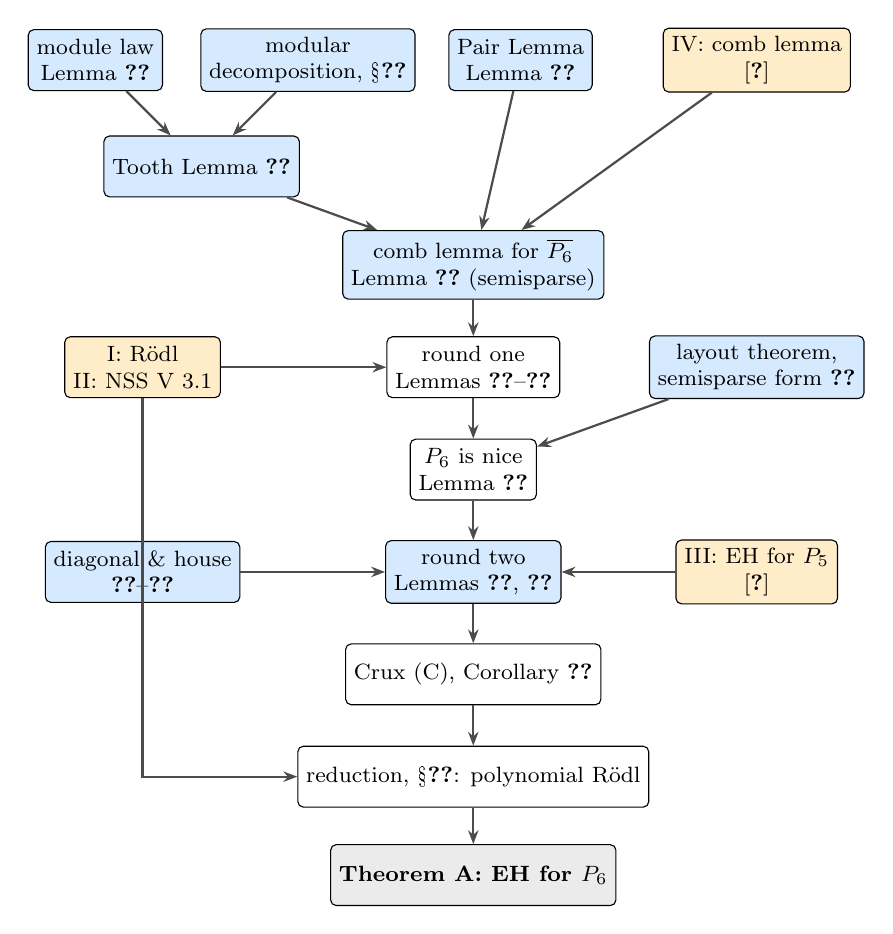
\begin{tikzpicture}[
  box/.style={draw,rounded corners=2pt,align=center,font=\footnotesize,minimum height=2.2em,inner sep=3pt},
  new/.style={box,fill=newpart},
  imp/.style={box,fill=imported},
  inh/.style={box,fill=white},
  arr/.style={-{Stealth[length=5pt]},thick,black!70}]
  \node[new] (ML) at (0,0) {module law\\ Lemma~\ref{lem:module}};
  \node[new] (MD) at (2.7,0) {modular\\decomposition, \S\ref{sec:md}};
  \node[new] (PL) at (5.4,0) {Pair Lemma\\ Lemma~\ref{lem:pair}};
  \node[imp] (IV) at (8.4,0) {IV: comb lemma\\ \cite{C5}};
  \node[new] (TL) at (1.35,-1.35) {Tooth Lemma~\ref{lem:tooth}};
  \node[new] (CL) at (4.8,-2.6) {comb lemma for $\cP$\\ Lemma~\ref{lem:comb} (semisparse)};
  \node[imp] (R12) at (0.6,-3.9) {I: R\"odl\\ II: NSS~V 3.1};
  \node[inh] (R1) at (4.8,-3.9) {round one\\ Lemmas~\ref{lem:r1step}--\ref{lem:r1blockade}};
  \node[new] (LT) at (8.4,-3.9) {layout theorem,\\ semisparse form~\ref{thm:layout}};
  \node[inh] (NI) at (4.8,-5.2) {$P_6$ is nice\\ Lemma~\ref{lem:nice}};
  \node[new] (HL) at (0.6,-6.5) {diagonal \& house\\ \ref{lem:diagonal}--\ref{cor:housefree}};
  \node[imp] (EH5) at (8.4,-6.5) {III: EH for $P_5$\\ \cite{NSS7}};
  \node[new] (R2) at (4.8,-6.5) {round two\\ Lemmas~\ref{lem:round2step}, \ref{lem:round2}};
  \node[inh] (CR) at (4.8,-7.8) {Crux (C), Corollary~\ref{cor:crux}};
  \node[inh] (C01) at (4.8,-9.1) {reduction, \S\ref{sec:c01}: polynomial R\"odl};
  \node[box,fill=black!8,font=\footnotesize\bfseries] (A) at (4.8,-10.35) {Theorem A: EH for $P_6$};
  \draw[arr] (ML) -- (TL); \draw[arr] (MD) -- (TL);
  \draw[arr] (TL) -- (CL); \draw[arr] (PL) -- (CL); \draw[arr] (IV) -- (CL);
  \draw[arr] (CL) -- (R1); \draw[arr] (R12) -- (R1);
  \draw[arr] (R1) -- (NI); \draw[arr] (LT) -- (NI);
  \draw[arr] (NI) -- (R2); \draw[arr] (HL) -- (R2); \draw[arr] (EH5) -- (R2);
  \draw[arr] (R2) -- (CR); \draw[arr] (CR) -- (C01);
  \draw[arr] (R12.south) |- (C01.west);
  \draw[arr] (C01) -- (A);
\end{tikzpicture}
\caption{Structure of the proof. Blue: proved here and specific to $\cP$ or new. Orange: the four
imported theorems (II is proved in the formalization). White: steps that follow~\cite{NSS7}, with constants recomputed.}
\label{fig:architecture}
\end{figure}

\setcounter{section}{-1}
\section{Preliminaries}\label{sec:prelim}

\subsection{Notation}
Graphs are finite and simple, $|G|=|V(G)|$, $N(v)$ is the neighbourhood of $v$, and $G[X]$ is the
subgraph induced on $X\subseteq V(G)$. We freely identify $X$ with $G[X]$. For disjoint $A,B$, $e(A,B)$ is
the number of edges between them. $A$ is \emph{complete} (\emph{anticomplete}) to $B$ if every (no) pair
$ab$ with $a\in A$, $b\in B$ is an edge. The pair is \emph{pure} if it is one of the two. A vertex is
\emph{mixed} on a set if it has both a neighbour and a non-neighbour there.

\begin{definition}[Sparsity]
Let $x\ge0$. A graph $G$ is \emph{$x$-sparse} if every vertex has at most $x|G|$ neighbours, and
\emph{$x$-restricted} if $G$ or $\Gbar$ is $x$-sparse. A set $X$ is $x$-sparse or $x$-restricted if $G[X]$
is. For disjoint $A,B$: $B$ is \emph{$x$-sparse to} $A$ if every vertex of $B$ has at most $x|A|$
neighbours in $A$, and $(A,B)$ is \emph{weakly $x$-sparse} if $e(A,B)\le x|A||B|$. If $B$ is $x$-sparse to
$A$ then $(A,B)$ is weakly $x$-sparse.
\end{definition}

\begin{definition}[Blockades]
For reals $k,w$, a \emph{$(k,w)$-blockade} is a sequence $(B_1,\dots,B_m)$ of pairwise disjoint sets
(\emph{blocks}, possibly empty) with $m\ge k$ and $|B_i|\ge w$ for all $i$. It is \emph{complete},
\emph{anticomplete} or \emph{pure} if every two blocks are complete, anticomplete or pure, respectively.
It is \emph{$x$-sparse} if $B_j$ is $x$-sparse to $B_i$ whenever $i<j$, and \emph{$x$-semisparse} if every
two blocks are complete or weakly $x$-sparse. A pure blockade is $0$-semisparse; an $x$-sparse blockade is
$x$-semisparse.
\end{definition}

A set $X$ is \emph{anticonnected} if $\Gbar[X]$ is connected, equivalently if every partition of $X$ into
two nonempty parts has a non-adjacent pair across. An \emph{anticomponent} of $X$ is the vertex set of a
component of $\Gbar[X]$. Distinct anticomponents of $X$ are complete to each other, and each anticomponent
is complete to the rest of $X$. We write $\hom(G)=\max(\alpha(G),\omega(G))=\hom(\Gbar)$. $P_k$ is the
path on $k$ vertices, $\cP$ is its complement for $k=6$, namely six vertices whose five non-adjacent pairs
form a path, and the \emph{house} is $\overline{P_5}$. Logarithms are to base $2$.

\subsection{The four imported theorems}\label{sec:imported}
We quote each result as stated in its source, together with the definitions it depends on, and then give
the Lean proposition that renders it (file \texttt{formal/EHP6/Imported.lean}). The main formal theorem
takes these four propositions as hypotheses. Theorem~\ref{imp:path} is proved in the formalization, so
the unconditional formal result assumes only the other three; see Section~\ref{sec:formal}. Each proposition is stated for
an arbitrary vertex set $S$ of a graph $G$, meaning the induced subgraph $G[S]$. This is equivalent to the source statement because induced
subgraphs of $H$-free graphs are $H$-free. In the Lean code, \lean{Free G H} means that $G$ has no induced
copy of $H$, \lean{Sparse G x S} means that every vertex of $S$ has at most $x|S|$ neighbours in $S$, and
\lean{Restricted G x S} means \lean{Sparse G x S} or \lean{Sparse Gᶜ x S}. Section~\ref{sec:formal} gives the
full definitions.

\begin{importedthm}[R\"odl~\cite{Rodl}; stated as {\cite[Theorem 1.3]{NSS7}}]\label{imp:rodl}
\emph{Source:} ``For every $\eps\in(0,1/2)$ and every graph $H$, there exists $\delta>0$ such that every
$H$-free graph $G$ has an $\eps$-restricted induced subgraph with at least $\delta|G|$ vertices.'' Here
$G$ is \emph{$\eps$-sparse} if its maximum degree is at most $\eps|G|$, and \emph{$\eps$-restricted} if one
of $G,\Gbar$ is $\eps$-sparse. We use it only for $H=\cP$ and write $\delta(\eps)$ for the constant.
\begin{lstlisting}
def RodlCoP6 : Prop := ∀ ε : ℝ, 0 < ε → ε < 1 / 2 → ∃ δ : ℝ, 0 < δ ∧
  ∀ (V : Type) [Fintype V] [DecidableEq V] (G : SimpleGraph V) [DecidableRel G.Adj],
    Free G P6ᶜ → ∀ S : Finset V, ∃ F ⊆ S, δ * S.card ≤ F.card ∧ Restricted G ε F
\end{lstlisting}
\end{importedthm}

\begin{importedthm}[{\cite[statement 3.1]{NSS5}}]\label{imp:path}
\emph{Source:} ``Let $P$ be a path with $k\ge2$ vertices, and let $0<y\le1/(60k)$. Let $G$ be a
$y^2$-sparse graph. Then either $G$ contains a copy of $P$, or $G$ contains an anticomplete
$(1/y,\lfloor y^2|G|\rfloor)$-blockade in $G$.'' In~\cite{NSS5} a blockade is a finite sequence of possibly
empty disjoint sets, and a $(k,w)$-blockade has length at least $k$ and width at least $w$, as above. A
``copy'' of $P$ is an induced copy: $H$-freeness in~\cite{NSS5} refers to induced subgraphs, and the
proof of~\cite[3.1]{NSS5} constructs an induced path. We use it for $P=P_6$, so $k=6$ and $y\le1/360$.
\begin{lstlisting}
def NssPath6 : Prop := ∀ y : ℝ, 0 < y → y ≤ 1 / 360 →
  ∀ (V : Type) [Fintype V] [DecidableEq V] (G : SimpleGraph V) [DecidableRel G.Adj]
    (S : Finset V), Sparse G (y ^ 2) S → ¬ ContainsInduced G P6 S →
      ∃ β : Blockade S (1 / y) (⌊y ^ 2 * S.card⌋₊ : ℝ), β.IsAnticomplete G
\end{lstlisting}
\emph{Proved in the formalization} (\texttt{formal/EHP6/NSSPath.lean}, for every $k\ge1$), following the
proof in~\cite{NSS5}. The only change is that the repeated removal of small sets with few neighbours
is replaced by a maximal family of such sets, which are pairwise disjoint and anticomplete; the maximality
gives the expansion property of the remaining vertices directly.
\end{importedthm}

\begin{importedthm}[Nguyen, Scott and Seymour~{\cite[Theorem 1.2]{NSS7}}]\label{imp:eh5}
\emph{Source:} ``$P_5$ satisfies the Erd\H{o}s--Hajnal conjecture,'' that is, there exists $c>0$ such that
every $P_5$-free graph $G$ has a clique or a stable set of size at least $|G|^{c}$. We fix such a
$\kappa>0$. Since $\hom(G)=\hom(\Gbar)$, every house-free graph $G$ also has $\hom(G)\ge|G|^{\kappa}$.
\begin{lstlisting}
def EhP5 : Prop := ∃ c : ℝ, 0 < c ∧
  ∀ (V : Type) [Fintype V] [DecidableEq V] (G : SimpleGraph V) [DecidableRel G.Adj],
    Free G P5 → ∃ T : Finset V, (IsCliqueF G T ∨ IsStableF G T) ∧ (Fintype.card V : ℝ) ^ c ≤ T.card
\end{lstlisting}
\end{importedthm}

\begin{importedthm}[the comb lemma; {\cite[Lemma 4.3]{NSS7}}, a special case of a lemma of~\cite{C5}]\label{imp:comb}
\emph{Source:} ``Let $G$ be a graph and let $A,B\subseteq V(G)$ be nonempty and disjoint, such that each
vertex in $A$ has at most $\Delta>0$ neighbours in $B$. Then either at most $20\sqrt{|B|\Delta}$ vertices
in $B$ have a neighbour in $A$; or for some integer $k\ge1$, there is a $(k,|B|/k^2)$-comb
$((a_i,B_i):i\in[k])$ in $G$ where $a_i\in A$ and $B_i\subset B$ for all $i\in[k]$.'' Here an
\emph{$(\ell,w)$-comb} is a sequence of pairs $((a_i,B_i):i\in[\ell])$ where $(B_1,\dots,B_\ell)$ is an
$(\ell,w)$-blockade, the $a_i$ are pairwise distinct, $\{a_1,\dots,a_\ell\},B_1,\dots,B_\ell$ are pairwise
disjoint, and for distinct $i,j$, $a_i$ is complete to $B_i$ and anticomplete to $B_j$. The symbol
$\subset$ in the source denotes inclusion; for $k=1$ it must allow $B_1=B$.
\begin{lstlisting}
def NssComb : Prop :=
  ∀ (V : Type) [Fintype V] [DecidableEq V] (G : SimpleGraph V) [DecidableRel G.Adj]
    (A B : Finset V) (Δ : ℝ), Disjoint A B → A.Nonempty → B.Nonempty → 0 < Δ →
    (∀ a ∈ A, ((nbrs G a B).card : ℝ) ≤ Δ) →
    (((B.filter (fun b => ∃ a ∈ A, G.Adj a b)).card : ℝ) ≤ 20 * Real.sqrt (B.card * Δ)) ∨
    (∃ ℓ : ℕ, 1 ≤ ℓ ∧ ∃ (a : Fin ℓ → V) (C : Fin ℓ → Finset V),
      Function.Injective a ∧ (∀ i, a i ∈ A) ∧ (∀ i, C i ⊆ B) ∧
      (∀ i j, i ≠ j → Disjoint (C i) (C j)) ∧
      (∀ i, (B.card : ℝ) / ℓ ^ 2 ≤ (C i).card) ∧
      (∀ i, ∀ c ∈ C i, G.Adj (a i) c) ∧
      (∀ i j, i ≠ j → ∀ c ∈ C j, ¬ G.Adj (a i) c))
\end{lstlisting}
The disjointness of the apexes from the teeth follows from $A\cap B=\emptyset$.
\end{importedthm}

\subsection{Two elementary lemmas of Nguyen, Scott and Seymour}
The proof also uses Lemmas 4.1 and 4.2 of~\cite{NSS7}. We prove both, since they are short and are
proved in the formalization. Lemma~\ref{lem:locate} is~\cite[Lemma 4.2]{NSS7} in the form of arXiv version~3
(February 2026), with the added hypothesis $A\ne\emptyset$: for $A=\emptyset\ne B$ the hypothesis holds
vacuously but the conclusion fails. This does not affect any use of it, here or in~\cite{NSS7}. The
revision of~\cite{NSS7} dated July 2026 states the lemma for all $x>0$ with the weaker bound
$|A'|\le2/x$; since we prove Lemma~\ref{lem:locate} below, nothing here depends on which version is used.

\begin{lemma}[{\cite[Lemma 4.1]{NSS7}}]\label{lem:cores}
Let $k\ge2$ be an integer and let $G$ be a graph all of whose anticomponents have fewer than $|G|/k$
vertices. Then $G$ has a complete $(k,|G|/k^2)$-blockade.
\end{lemma}
\begin{proof}
Let $n=|G|$, $w=n/k^2$, $c=n/k$. Distinct anticomponents are complete to each other, so if
$\cG_1,\dots,\cG_k$ are disjoint collections of anticomponents, the unions $\bigcup\cG_1,\dots,\bigcup\cG_k$
are pairwise complete. From any
collection of anticomponents of total size at least $w$ we can pick a subcollection of total size in
$[w,w+c)$: add members one at a time until the total reaches $w$, and use that every member has size
$<c$. Pick such subcollections $\cG_1,\cG_2,\dots$ greedily from the anticomponents not yet used. After
$j\le k-1$ steps at most $(k-1)(w+c)=n-n/k^2$ vertices are used, so the remaining anticomponents have
total size at least $w$ and step $j+1$ is possible. The unions of $\cG_1,\dots,\cG_k$ form a complete
$(k,n/k^2)$-blockade.
\end{proof}

Applied to $\Gbar$: if every component of $G$ has fewer than $|G|/k$ vertices, then $G$ has an
anticomplete $(k,|G|/k^2)$-blockade.

\begin{lemma}[{cf.~\cite[Lemma 4.2]{NSS7}}]\label{lem:locate}
Let $x\in(0,\frac12)$, let $A\ne\emptyset$ and $B$ be sets of vertices, and suppose every vertex of $B$ has
at least $x|A|$ neighbours in $A$. Then there is $A'\subseteq A$ with $|A'|\le1/x$ such that at least
$|B|/2$ vertices of $B$ have a neighbour in $A'$.
\end{lemma}
\begin{proof}
Let $U\subseteq B$. Counting edges, $\sum_{a\in A}|N(a)\cap U|=\sum_{b\in U}|N(b)\cap A|\ge x|A||U|$, so
some $a\in A$ has at least $x|U|$ neighbours in $U$. Choose $a_1,a_2,\dots,a_t$ greedily, each covering an
$x$-fraction of the vertices of $B$ not yet covered, where $t=\lfloor1/x\rfloor$. At most $(1-x)^t|B|$
vertices remain uncovered. As $x<\frac12$, $t\ge2$ and $x>1/(t+1)$, so $1-x<t/(t+1)$, and Bernoulli's
inequality $(1+1/t)^t\ge2$ gives $(1-x)^t\le(t/(t+1))^t\le\frac12$. Take $A'=\{a_1,\dots,a_t\}$.
\end{proof}

\begin{lemma}\label{lem:anticonn}
If $D$ is anticonnected and $1\le b\le|D|$, then $D$ contains an anticonnected set of exactly $b$
vertices.
\end{lemma}
\begin{proof}
Start from a single vertex. If $B\subsetneq D$ is anticonnected, anticonnectivity of $D$ applied to the
partition $(B,D\setminus B)$ gives $p\in B$ and $q\in D\setminus B$ with $pq\notin E(G)$, and $B\cup\{q\}$
is anticonnected.
\end{proof}

\subsection{Modular decomposition}\label{sec:md}
Let $Y$ be a set of vertices. A \emph{module} of $G[Y]$ is a set $M\subseteq Y$ such that every vertex of
$Y\setminus M$ is complete or anticomplete to $M$. A module is \emph{strong} if it overlaps no other
module, where two sets overlap if they meet and neither contains the other. The following facts are
standard (Gallai~\cite{Gallai}); the forms used below are proved in the formalization. The strong modules
of $G[Y]$ form a laminar family containing $Y$ and all singletons, that is, a rooted tree under inclusion.
The \emph{children} of a strong module $N$ with $|N|\ge2$ are the maximal strong modules properly
contained in $N$, and they partition $N$. There are three kinds of node:
\begin{itemize}[leftmargin=1.5em]
\item $N$ is \emph{parallel} if $G[N]$ is disconnected; then its children are the components of $G[N]$;
\item $N$ is \emph{series} if $\Gbar[N]$ is disconnected; then its children are the anticomponents of
  $N$;
\item $N$ is \emph{prime} if $G[N]$ and $\Gbar[N]$ are both connected; then the quotient graph on the
  children (two children adjacent if complete to each other) is prime, that is, it has at least four
  vertices and no modules other than the trivial ones.
\end{itemize}
A module of $G[N]$ for a module $N$ of $G[Y]$ is a module of $G[Y]$.

\begin{lemma}[MD1]\label{lem:md1}
Disjoint modules $A,B$ of $G[Y]$ are pure to each other.
\end{lemma}
\begin{proof}
Each $a\in A$ lies outside $B$, so it is complete or anticomplete to $B$. If $a_1\in A$ were complete and
$a_2\in A$ anticomplete to $B$, any $b\in B$ would be mixed on the module $A$, impossible as $b\notin A$.
\end{proof}

\begin{lemma}[MD2]\label{lem:md2}
If $N$ is a prime node, every module $X$ of $G[N]$ equals $N$ or is contained in one child of $N$.
\end{lemma}
\begin{proof}
Let $I$ be the set of children meeting $X$, and suppose $|I|\ge2$. For a child $C\notin I$ and $c\in C$,
the adjacency of $c$ to a child $M\in I$ equals its adjacency to $X\cap M$ ($M$ is a module and
$c\notin M$), which equals its adjacency to $X$ ($X$ is a module and $c\notin X$). Hence $I$ is a module
of the prime quotient, and since $|I|\ge2$ it contains all children. If some child $M_1\not\subseteq X$,
take $m\in M_1\setminus X$. For every other child $M$ the adjacency of $m$ to $M$ equals its adjacency to
$X\cap M$, which equals its adjacency to $X$. So in the quotient, $M_1$ is complete or anticomplete to all
other children, and these, at least three of them, form a nontrivial module of the prime quotient, a
contradiction. Hence every child lies in $X$, and $X=N$.
\end{proof}

\section{The local lemmas}\label{sec:local}
These three lemmas are the only places where $\cP$-freeness is used, apart from the imported
Theorems~\ref{imp:rodl} and~\ref{imp:path}. Each is proved by exhibiting an induced $\cP$
(Figure~\ref{fig:certificates}).

\subsection{The module law}

\begin{figure}[ht]
\centering
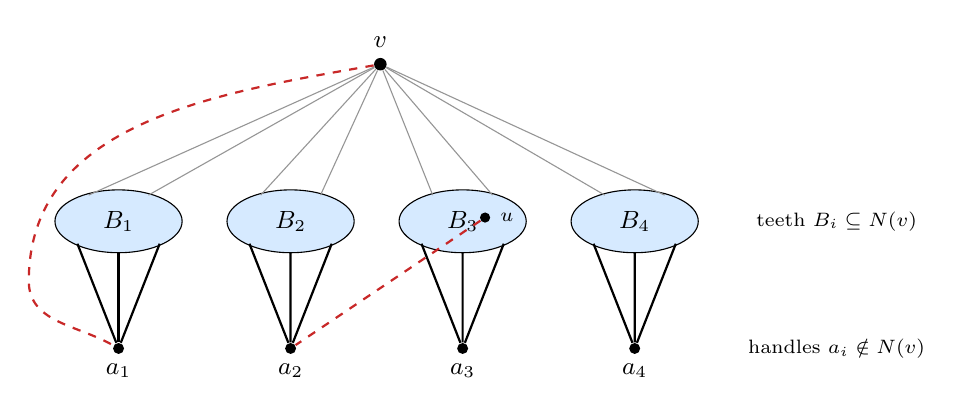
\begin{tikzpicture}[scale=0.95,every node/.style={font=\small}]
  \node[circle,fill,inner sep=1.6pt,label=above:$v$] (v) at (3.5,2.3) {};
  \foreach \i/\x in {1/0,2/2.3,3/4.6,4/6.9} {
    \draw[fill=newpart] (\x,0.2) ellipse (0.85 and 0.42);
    \node at (\x,0.2) {$B_{\i}$};
    \node[circle,fill,inner sep=1.4pt,label=below:$a_{\i}$] (a\i) at (\x,-1.5) {};
    \draw[thick] (a\i) -- (\x-0.55,-0.1); \draw[thick] (a\i) -- (\x+0.55,-0.1); \draw[thick] (a\i) -- (\x,-0.22);
    \draw[edgegrey] (v) -- (\x-0.4,0.55); \draw[edgegrey] (v) -- (\x+0.4,0.55);
  }
  \draw[nonedge,dashed,thick] (v) to[out=190,in=90] (-1.2,-0.6) to[out=-90,in=150] (a1);
  \node[circle,fill,inner sep=1.3pt,label={[font=\scriptsize]right:$u$}] (u) at (4.9,0.25) {};
  \draw[nonedge,dashed,thick] (u) -- (a2);
  \node[font=\scriptsize,align=left] at (9.6,0.2) {teeth $B_i\subseteq N(v)$};
  \node[font=\scriptsize,align=left] at (9.6,-1.5) {handles $a_i\notin N(v)$};
\end{tikzpicture}
\caption{A comb with root $v$. Each handle $a_i$ is complete to its own tooth $B_i$ and anticomplete
to the other teeth, and $v$ is complete to every tooth and non-adjacent to the handles. The module law
applies to $Z=B_i$ and a vertex $u$ of another tooth $B_j$: $u\sim v$ and $u\not\sim a_i$.}
\label{fig:comb}
\end{figure}

\begin{lemma}[module law]\label{lem:module}
Let $G$ be $\cP$-free, let $v,a$ be non-adjacent vertices, let $Z\subseteq N(v)\cap N(a)$, and let
$u\notin Z$ with $u\sim v$ and $u\not\sim a$. Then every anticomponent $K$ of $N(u)\cap Z$ is a module of
$G[Z]$.
\end{lemma}
\begin{proof}
Vertices of $(N(u)\cap Z)\setminus K$ lie in other anticomponents of $N(u)\cap Z$, so they are complete to
$K$. Suppose $y\in Z\setminus N(u)$ is mixed on $K$. Since $K$ is anticonnected and $N(y)\cap K$ and
$K\setminus N(y)$ are both nonempty, there are $w\in N(y)\cap K$ and $z\in K\setminus N(y)$ with
$w\not\sim z$. The six vertices $v,a,u,y,z,w$ are distinct: $v,a\notin Z$ because $Z\subseteq N(v)\cap
N(a)$, and $u\notin Z$. Their adjacent pairs are $v$ with $u,y,z,w$ ($u\sim v$ by hypothesis, and
$y,z,w\in Z$); $a$ with $y,z,w$; $u$ with $z,w$ (as $z,w\in K\subseteq N(u)$); and $yw$. The non-adjacent
pairs are $va, au, uy, yz, zw$, a path. So $v,a,u,y,z,w$ induce $\cP$, a contradiction.
\end{proof}

\subsection{Mixed-vertex patterns are house-free}
Throughout this subsection $B_1,\dots,B_\ell$ is a \emph{block system}: disjoint anticonnected sets of the
same size $W\ge1$ such that, for some $x\in(0,\frac12)$, every two of them are complete or $x$-sparse to
each other in both directions. Since $x<1$, no pair is both. The \emph{pattern graph} $J$ on $[\ell]$ has
$ij\in E(J)$ if and only if $B_i$ is complete to $B_j$.

\begin{lemma}[diagonal lemma]\label{lem:diagonal}
Let $G$ be $\cP$-free, and let $b,c,d,e,f$ be indices such that $B_b$ is complete to $B_d,B_e,B_f$, $B_c$ is
complete to $B_e,B_f$, $B_d$ is complete to $B_f$, and the pairs $(b,c),(c,d),(d,e),(e,f)$ are not
complete (hence $x$-sparse). Then $B_e$ is anticomplete to $B_f$.
\end{lemma}
\begin{proof}
Suppose $x_0\in B_e$ has a neighbour in $B_f$. Since $|N(x_0)\cap B_f|\le xW<W$, $x_0$ also has a
non-neighbour in $B_f$, and since $B_f$ is anticonnected there are $p\in N(x_0)\cap B_f$ and $q\in
B_f\setminus N(x_0)$ with $p\not\sim q$. Take $u_b\in B_b$, then $u_c\in B_c\setminus N(u_b)$ (possible as
$|N(u_b)\cap B_c|\le xW<W$), then $u_d\in B_d\setminus(N(x_0)\cup N(u_c))$ (possible as each of $x_0,u_c$
has at most $xW$ neighbours in $B_d$ and $2xW<W$). Among $p,q,x_0,u_d,u_c,u_b$ the adjacent pairs are
$px_0$ (by choice); $p$ and $q$ with $u_d,u_c,u_b$ (as $B_f$ is complete to $B_d,B_c,B_b$); $x_0$ with
$u_c,u_b$ (as $B_e$ is complete to $B_c,B_b$); and $u_du_b$ (as $B_d$ is complete to $B_b$). The non-adjacent
pairs are $pq,qx_0,x_0u_d,u_du_c,u_cu_b$, a path. This is an induced $\cP$, a contradiction.
\end{proof}

\begin{figure}[ht]
\centering
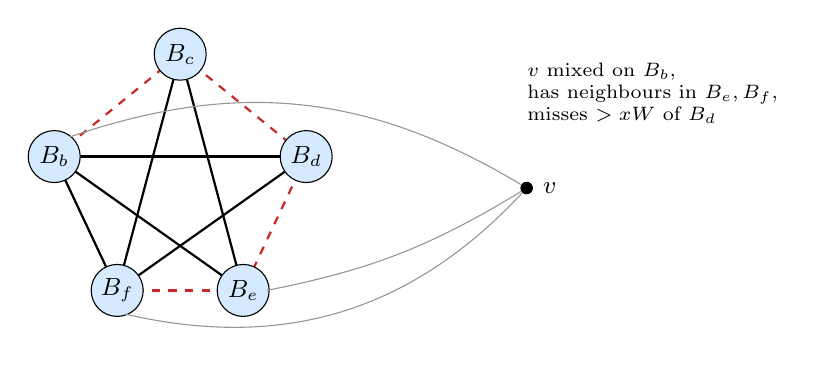
\begin{tikzpicture}[scale=1.0,every node/.style={font=\small}]
  \coordinate (b) at (0,0); \coordinate (c) at (1.6,1.3); \coordinate (d) at (3.2,0);
  \coordinate (e) at (2.4,-1.7); \coordinate (f) at (0.8,-1.7);
  \foreach \p/\q in {b/d,b/e,b/f,c/e,c/f,d/f} \draw[thick] (\p) -- (\q);
  \foreach \p/\q in {b/c,c/d,d/e,e/f} \draw[nonedge,dashed,thick] (\p) -- (\q);
  \foreach \p in {b,c,d,e,f} {\draw[fill=newpart] (\p) circle (0.33); \node at (\p) {$B_{\p}$};}
  \node[circle,fill,inner sep=1.6pt,label=right:$v$] (v) at (6.0,-0.4) {};
  \draw[edgegrey] (v) to[bend right=25] ($(b)+(0.2,0.25)$);
  \draw[edgegrey] (v) to[bend left=10] ($(e)+(0.3,0)$);
  \draw[edgegrey] (v) to[bend left=30] ($(f)+(0.1,-0.3)$);
  \node[font=\scriptsize,align=left] at (7.6,0.8) {$v$ mixed on $B_b$,\\ has neighbours in $B_e,B_f$,\\ misses $>xW$ of $B_d$};
\end{tikzpicture}
\caption{A house in the pattern graph: solid pairs are complete, dashed pairs are not complete. The four
dashed pairs $bc,cd,de,ef$ form a path, so the pattern is the complement of $P_5$. By the house lemma no
outside vertex $v$ can be lightly mixed on all five blocks.}
\label{fig:house}
\end{figure}

\begin{lemma}[house lemma]\label{lem:house}
Let $G$ be $\cP$-free and let $b,c,d,e,f$ be as in Lemma~\ref{lem:diagonal}. Then no vertex
$v\notin\bigcup_iB_i$ has all of the following: a neighbour and a non-neighbour in $B_b$, a neighbour in
$B_e$, a neighbour in $B_f$, and more than $xW$ non-neighbours in $B_d$.
\end{lemma}
\begin{proof}
Suppose $v$ has them. Take $x_e\in N(v)\cap B_e$ and $x_f\in N(v)\cap B_f$; by Lemma~\ref{lem:diagonal},
$x_e\not\sim x_f$. By anticonnectivity of $B_b$ there are $p_b\in N(v)\cap B_b$ and $q_b\in B_b\setminus
N(v)$ with $p_b\not\sim q_b$. Take $u_d\in B_d\setminus(N(v)\cup N(x_e))$, possible because
$|N(x_e)\cap B_d|\le xW<|B_d\setminus N(v)|$. Among $p_b,q_b,v,u_d,x_e,x_f$ the adjacent pairs are $p_b$
and $q_b$ with $u_d,x_e,x_f$ (as $B_b$ is complete to $B_d,B_e,B_f$); $v$ with $p_b,x_e,x_f$; and $u_dx_f$ (as
$B_d$ is complete to $B_f$). The non-adjacent pairs are $p_bq_b,q_bv,vu_d,u_dx_e,x_ex_f$, a path. This is
an induced $\cP$, a contradiction.
\end{proof}

For a vertex $v\notin\bigcup_iB_i$ let $I(v)=\{i:0<|N(v)\cap B_i|<W/2\}$ be the set of blocks on which $v$
is \emph{lightly mixed}, and $J_v=J[I(v)]$.

\begin{corollary}\label{cor:housefree}
Let $G$ be $\cP$-free and $v\notin\bigcup_iB_i$. Then $J_v$ is house-free. Consequently there is
$R\subseteq I(v)$ with $|R|\ge|I(v)|^{\kappa}$ whose blocks are pairwise complete or pairwise not complete.
\end{corollary}
\begin{proof}
An induced house in $J_v$ on $b,c,d,e,f$, with non-edges $bc,cd,de,ef$ (the complement of the path
$b$--$c$--$d$--$e$--$f$), has exactly the completeness pattern of Lemma~\ref{lem:diagonal}. The vertex $v$ is
mixed on $B_b$ and has neighbours in $B_e$ and $B_f$, and $|B_d\setminus N(v)|>W/2>xW$. This contradicts
Lemma~\ref{lem:house}. For the second statement note that the complement of $J_v$ is $P_5$-free, so by
Theorem~\ref{imp:eh5} it has a clique or a stable set with at least $|I(v)|^\kappa$ vertices, and so does
$J_v$. A clique of $J_v$ is a set of pairwise complete blocks, and a stable set is a set of pairwise
non-complete blocks.
\end{proof}

\section{The Tooth Lemma and the Pair Lemma}\label{sec:tooth}

The Tooth Lemma is the main new structural result. Its input is a set $Y$, which will be a tooth of a
comb, together with a set $U$ of outside vertices that see $Y$ only through modules, as the module law
guarantees. Its output is a long pure or complete blockade inside $Y$, or a large subset $Y'\subseteq Y$
that each $u\in U$ sees completely or very sparsely.

\begin{lemma}[Tooth Lemma]\label{lem:tooth}
Let $0<x\le2^{-20}$, let $k$ be an integer with $2^{16}\le k\le2x^{-1/2}$, let $Y$ be a set of $n:=|Y|\ge
16x^{-3}$ vertices, and let $U$ be a set of vertices such that for every $u\in U$ every anticomponent of
$N(u)\cap Y$ is a module of $G[Y]$. Then $G[Y]$ contains one of the following:
\begin{enumerate}[label=(TL\arabic*),leftmargin=3.2em]
\item a pure $(K,n/K^4)$-blockade, for some integer $K$ with $K^4\ge k$ and $K\le1/x$;
\item a pure $(L,n/(2k))$-blockade, for an integer $L$ with $(8L)^4\le k^3\le(9L)^4$;
\item a complete or anticomplete $(\floor{1/x},x^2n/k)$-blockade;
\item a complete $(\floor{1/(xk)},x^3n/4)$-blockade;
\item a set $Y'\subseteq Y$ with $|Y'|\ge n/k$ such that for every $u\in U$, either $Y'\subseteq N(u)$ or
  $|N(u)\cap Y'|<x|Y'|/4$.
\end{enumerate}
\end{lemma}

In (TL1) the length is at least $k^{1/4}$, and in (TL2) it lies between $k^{3/4}/9$ and $k^{3/4}/8$.
Lengths are written without roots because this is how they are stated in Lean.

\begin{proof}
Note that $k\le2x^{-1/2}$ gives $k^2x\le4$ and $xk\le2x^{1/2}\le2^{-9}$. Set
\[
s:=x^2n/4,\qquad t:=n/k,\qquad K_1:=\floor{1/x}.
\]
Then $s\ge4/x>1$, and $s\le t$ because $xk\le4$. Let $\cL$ be the set of strong modules of $G[Y]$ with at
least $s$ vertices. It contains $Y$ and is closed upwards in the tree of strong modules. An \emph{atom} is
a child of a member of $\cL$ that is not itself in $\cL$, so every atom has fewer than $s$ vertices. For
$N\in\cL$ let $S(N)$ be the union of the atom children of $N$, the \emph{layer} of $N$. We use three facts.

\begin{enumerate}[label=(F\arabic*),leftmargin=2.5em]
\item \emph{The layers $S(N)$, $N\in\cL$, partition $Y$.} For $v\in Y$ let $N_v$ be a minimal member of
  $\cL$ containing $v$. The child of $N_v$ containing $v$ is not in $\cL$, so $v\in S(N_v)$. Suppose $v\in
  S(N)\cap S(N')$ with $N\neq N'$. By laminarity one of them, say $N'$, is strictly inside the other.
  The child $C$ of $N$ containing $v$ and the strong module $N'$ both contain $v$, so they are nested.
  $C\subsetneq N'\subsetneq N$ would contradict $C$ being a child, so $N'\subseteq C$ and $|C|\ge|N'|\ge s$,
  contradicting that $C$ is an atom.
\item \emph{Let $N\in\cL$, $u\in U$ and $T:=N(u)\cap Y$. Each anticomponent $A$ of $G[T]$ satisfies
  $A\supseteq N$, or $A\cap N=\emptyset$, or $A\subsetneq N$.} This holds because $A$ is a module of $G[Y]$
  by hypothesis and $N$ is strong. In the third case, if $N$ is prime, Lemma~\ref{lem:md2} puts $A$ inside
  a single child of $N$.
\item \emph{If $N\supsetneq N'$ are in $\cL$, then $S(N)\cap N'=\emptyset$, and every vertex of $Y\setminus
  N'$ is complete or anticomplete to $N'$.} The first part is the argument of (F1), and the second holds
  because $N'$ is a module.
\end{enumerate}

\emph{Step 1: an antichain bound.} We use the following counting fact. Let $2\le K_0\le K_1$ and $M\ge0$,
and let $\cA$ be a family of sets, each of size at most $M$, such that for every integer
$K\in[K_0,K_1]$ fewer than $K$ members of $\cA$ have size at least $n/K^4$. Then
\begin{equation}\label{eq:antichain}
\sum_{A\in\cA}|A|\;\le\;(K_0-1)M+\frac{n}{K_0-1}+|\cA|\,\frac{n}{K_1^4}.
\end{equation}
Indeed, fewer than $K_0$ members have size at least $n/K_0^4$, and each has size at most $M$. For
$K_0\le K<K_1$, at most $K$ members have size in $[n/(K+1)^4,n/K^4)$, contributing at most $n/K^3$. The
remaining members have size below $n/K_1^4$. Finally $\sum_{K\ge K_0}K^{-3}\le\sum_{K\ge
K_0}\bigl(\frac1{K-1}-\frac1K\bigr)=\frac1{K_0-1}$.

Let $K_0$ be the least integer with $K_0^4\ge k$ and put $a:=K_0-1$. Then $a^4<k$ and, since $k\ge2^{16}$,
$a\ge15$. Moreover $K_0\le K_1$: from $a^8<k^2\le4/x$ and $a^7\ge8$ we get $8ax\le a^8x<4$, so $(a+1)x\le
2ax<1$.

\emph{Step 2: a heavy chain.} Let $\cL^*:=\{N\in\cL:|N|\ge t\}$ and let $\mathcal M$ be the set of minimal
members of $\cL^*$. They are pairwise disjoint modules of size at least $t\ge n/K_0^4$. So if $|\mathcal
M|\ge K_0$, any $K_0$ of them form a pure $(K_0,n/K_0^4)$-blockade by Lemma~\ref{lem:md1}, which is (TL1).
Assume $|\mathcal M|\le a$.

Let $\mathcal X$ be the set of maximal members of $\cL\setminus\cL^*$. They are pairwise disjoint and
have sizes in $[s,t)$, so $|\mathcal X|\le n/s$. If for some $K\in[K_0,K_1]$ at least $K$ of them have size
at least $n/K^4$, those $K$ sets form a pure $(K,n/K^4)$-blockade, which is (TL1). Otherwise
\eqref{eq:antichain} with $M=t$ gives
\[
\sum_{A\in\mathcal X}|A|\le a\frac nk+\frac na+\frac ns\cdot\frac n{K_1^4}
\le\frac{n}{a^3}+\frac n{15}+\frac{4}{x^2}\cdot16x^4n\le\Bigl(\frac1{3375}+\frac1{15}+2^{-34}\Bigr)n\le\frac n4,
\]
using $a^4<k$, $a\ge15$, $K_1\ge1/(2x)$ and $x\le2^{-20}$. Every member of $\cL\setminus\cL^*$ lies inside a
member of $\mathcal X$, and layers are disjoint, so the layers of members of $\cL\setminus\cL^*$ have total
size at most $n/4$. By (F1),
\[
\sum_{N\in\cL^*}|S(N)|\;\ge\;\frac{3n}4 .
\]
Every $N\in\cL^*$ contains a member of $\mathcal M$. Summing over $m\in\mathcal M$ and using $|\mathcal M|\le a$,
there is $m\in\mathcal M$ such that the family $\mathcal C:=\{N\in\cL^*:N\supseteq m\}$ satisfies
\[
\sum_{N\in\mathcal C}|S(N)|\;\ge\;\frac{3n}{4a}.
\]
Its members all contain $m$, so by laminarity $\mathcal C$ is a chain.

\emph{Step 3: a thick layer.} Suppose $|S(N)|\ge t$ for some $N\in\mathcal C$, and put $S:=S(N)$.
\begin{itemize}[leftmargin=1.5em]
\item \emph{$G[N]$ disconnected.} The children of $N$ are its components, so each component of $G[S]$ is
  an atom and has fewer than $s$ vertices. Since $s=x^2n/4\le xt\le|S|/K_1$, Lemma~\ref{lem:cores}
  applied in the complement gives an anticomplete $(K_1,|S|/K_1^2)$-blockade, and $|S|/K_1^2\ge
  x^2t=x^2n/k$. This is (TL3).
\item \emph{$\Gbar[N]$ disconnected.} The same argument with anticomponents gives a complete blockade: (TL3).
\item \emph{$N$ prime.} Let $K':=\floor{1/(xk)}\ge2$. Let $u\in U$ with $S\not\subseteq N(u)$ and
  $r:=|N(u)\cap S|\ge x|S|/4$, and let $T:=N(u)\cap Y$. Let $A$ be an anticomponent of $G[T]$ meeting $S$.
  If $A\supseteq N$ then $S\subseteq N(u)$, which is excluded, and $A\cap N=\emptyset$ is impossible. So by
  (F2) $A$ lies in a single child of $N$, and since it meets $S$, that child is an atom. Thus $N(u)\cap S$
  is a union of anticomponents of $G[T]$, each inside an atom. These are the anticomponents of $G[N(u)\cap
  S]$, and each has fewer than $s$ vertices. Now $r/K'\ge r\,xk\ge\frac{xt}4xk=s$, so
  Lemma~\ref{lem:cores} gives a complete $(K',r/K'^2)$-blockade, and $r/K'^2\ge\frac{xt}{4}(xk)^2\ge
  x^3n/4$. This is (TL4). If no such $u$ exists, $Y':=S$ satisfies (TL5).
\end{itemize}

\emph{Step 4: all layers thin.} Otherwise $|S(N)|<t$ for all $N\in\mathcal C$. Let $L$ be the largest
integer with $(8L)^4\le k^3$. Then $L\ge8$ and $k^3<(8L+8)^4\le(9L)^4$, as required in (TL2). Since
$(8La)^4\le k^3a^4<k^4$, we have $8La<k$ and so
\[
2Lt=\frac{2Ln}{k}\le\frac{3n}{4a}\le\sum_{N\in\mathcal C}|S(N)| .
\]
For $N\in\mathcal C$ let $P(N):=\sum_{N'\in\mathcal C,\,N'\supseteq N}|S(N')|$ be the layer mass from the top
of the chain down to $N$. For $0\le j<L$ let the \emph{chunk} $\Gamma_j$ be the union of the layers $S(N)$
with $2jt<P(N)\le2(j+1)t$. For every $\theta\le\sum_{N\in\mathcal C}|S(N)|$, the layers with $P(N)\le\theta$
have total size in $(\theta-t,\theta]$, because each layer has fewer than $t$ vertices. Taking
$\theta=2jt$ and $\theta=2(j+1)t$ shows that every chunk has more than $t$ vertices. If $j<j'$, every chain
member contributing to $\Gamma_{j'}$ lies strictly inside every chain member contributing to $\Gamma_j$:
its $P$-value is larger, and $P$ can only grow down the chain.

Say that $v\in Y$ has \emph{type~1} if $v$ is complete to every $N'\in\mathcal C$ with $v\notin N'$. A
vertex $v$ without type~1 is anticomplete to every such $N'$. To see this, take a member $N''\not\ni v$
to which $v$ is not complete; by (F3) $v$ is anticomplete to $N''$. Any other $N'\not\ni v$ is
comparable with $N''$, and $v$ is complete or anticomplete to it. If $N'\subseteq N''$, then $v$ is
anticomplete to $N'$. If $N'\supseteq N''$, then $v$ has a non-neighbour in $N''\subseteq N'$, so again
$v$ is anticomplete to $N'$. Now let $v\in S(N)\subseteq\Gamma_j$ and $w\in S(N')\subseteq\Gamma_{j'}$ with
$j<j'$. Then $N'\subsetneq N$, so $v\notin N'$ by (F3), and $v$ is adjacent to $w$ exactly when $v$ has
type~1. Let $\Gamma'_j\subseteq\Gamma_j$ be the vertices of the majority type, so $|\Gamma'_j|\ge t/2=n/(2k)$.
Then $(\Gamma'_0,\dots,\Gamma'_{L-1})$ is a pure $(L,n/(2k))$-blockade: (TL2).
\end{proof}

\begin{figure}[ht]
\centering
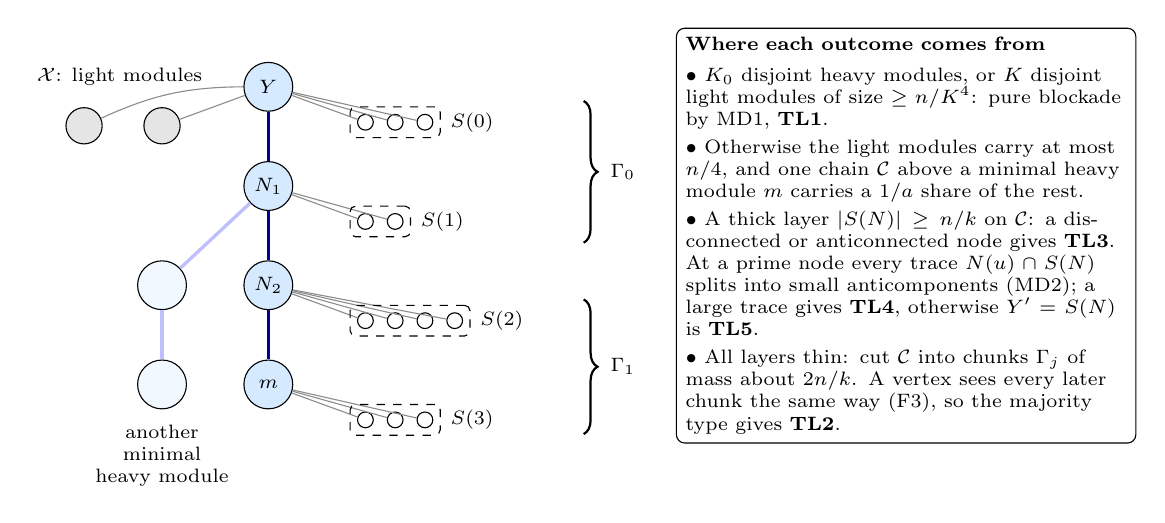
\begin{tikzpicture}[scale=0.9,
  heavy/.style={circle,draw,fill=newpart,minimum size=0.62cm,inner sep=0pt,font=\scriptsize},
  light/.style={circle,draw,fill=black!10,minimum size=0.46cm,inner sep=0pt},
  atom/.style={circle,draw,fill=white,minimum size=0.2cm,inner sep=0pt}]
  % the heavy chain C
  \foreach \t/\lab in {0/Y,1/N_1,2/N_2,3/m} \node[heavy] (N\t) at (0,-1.4*\t) {$\lab$};
  \foreach \t/\u in {0/1,1/2,2/3} \draw[very thick,blue!60!black] (N\t) -- (N\u);
  % atoms and layers
  \foreach \t/\mm in {0/3,1/2,2/4,3/3} {
    \foreach \j in {1,...,\mm} {\node[atom] (a\t\j) at (0.95+0.42*\j,-1.4*\t-0.5) {};
      \draw[black!45] (N\t) -- (a\t\j);}
    \node[draw,dashed,rounded corners=2pt,fit=(a\t1)(a\t\mm),inner sep=2.5pt,
      label={[font=\scriptsize]right:$S(\t)$}] {};
  }
  % other members of L*
  \node[heavy,fill=newpart!35] (H1) at (-1.5,-2.8) {};
  \draw[very thick,blue!25] (N1) -- (H1);
  \node[heavy,fill=newpart!35] (H2) at (-1.5,-4.2) {};
  \draw[very thick,blue!25] (H1) -- (H2);
  \node[font=\scriptsize,align=center,text width=1.8cm] at (-1.5,-5.2) {another minimal heavy module};
  % light members
  \node[light] (L0) at (-1.5,-0.55) {}; \draw[black!45] (N0) -- (L0);
  \node[light] (L1) at (-2.6,-0.55) {}; \draw[black!45] (N0) to[bend right=12] (L1);
  \node[font=\scriptsize,align=center] at (-2.1,0.15) {$\mathcal X$: light modules};
  % chunks
  \draw[decorate,decoration={brace,amplitude=5pt},thick] (4.45,-0.2) -- (4.45,-2.2)
    node[midway,right=6pt,font=\scriptsize] {$\Gamma_0$};
  \draw[decorate,decoration={brace,amplitude=5pt},thick] (4.45,-3.0) -- (4.45,-4.9)
    node[midway,right=6pt,font=\scriptsize] {$\Gamma_1$};
  % outcome panel
  \node[draw,rounded corners=3pt,align=left,font=\scriptsize,text width=5.6cm] at (9.0,-2.1) {%
  \textbf{Where each outcome comes from}\\[3pt]
  $\bullet$ $K_0$ disjoint heavy modules, or $K$ disjoint light modules of size $\ge n/K^4$: pure
  blockade by MD1, \textbf{TL1}.\\[2pt]
  $\bullet$ Otherwise the light modules carry at most $n/4$, and one chain $\mathcal C$ above a minimal
  heavy module $m$ carries a $1/a$ share of the rest.\\[2pt]
  $\bullet$ A thick layer $|S(N)|\ge n/k$ on $\mathcal C$: a disconnected or anticonnected node gives
  \textbf{TL3}. At a prime node every trace $N(u)\cap S(N)$ splits into small anticomponents (MD2); a
  large trace gives \textbf{TL4}, otherwise $Y'=S(N)$ is \textbf{TL5}.\\[2pt]
  $\bullet$ All layers thin: cut $\mathcal C$ into chunks $\Gamma_j$ of mass about $2n/k$. A vertex sees
  every later chunk the same way (F3), so the majority type gives \textbf{TL2}.};
\end{tikzpicture}
\caption{The proof of the Tooth Lemma. Circles are strong modules of $G[Y]$ with at least $s=x^2n/4$
vertices. Blue: heavy modules, with at least $t=n/k$ vertices; the dark path is the chain $\mathcal C$ of
heavy modules above one minimal heavy module $m$. Grey: light modules. Small white circles are atoms,
and the dashed box $S(i)$ is the layer of the $i$-th member of the chain.}
\label{fig:tooth}
\end{figure}

\begin{lemma}[Pair Lemma]\label{lem:pair}
Let $Y_1,Y_2$ be sets of vertices and $\theta>0$. Suppose every $w\in Y_1$ has
$Y_2\subseteq N(w)$ or $|N(w)\cap Y_2|<\theta|Y_2|$, and every $u\in Y_2$ has $Y_1\subseteq N(u)$ or
$|N(u)\cap Y_1|<\theta|Y_1|$. Then $(Y_1,Y_2)$ is complete or weakly $2\theta$-sparse.
\end{lemma}
\begin{proof}
Let $F:=\{u\in Y_2:Y_1\subseteq N(u)\}$. If $|F|\ge\theta|Y_2|$, then every $w\in Y_1$ has at least
$\theta|Y_2|$ neighbours in $Y_2$, so $Y_2\subseteq N(w)$ and the pair is complete. Otherwise
$e(Y_1,Y_2)<|F||Y_1|+|Y_2|\,\theta|Y_1|<2\theta|Y_1||Y_2|$.
\end{proof}

\section{The comb lemma for \texorpdfstring{$\cP$}{co-P6}}\label{sec:comb}

This section replaces~\cite[Lemma 5.2]{NSS7}, the step where the proof for $P_5$ uses that the teeth of a
comb are pure to each other. Lemma~\ref{lem:comb} has the same three outcomes, except that the blockade
in outcome (ii) is only semisparse.

\begin{lemma}\label{lem:comb}
Let $0<x\le y\le2^{-64}$, and let $G$ be a $y^3$-sparse $\cP$-free graph with $|G|\ge x^{-18}$. Then one
of the following holds:
\begin{enumerate}[label=(\roman*)]
\item $G$ is $2y^4$-sparse;
\item for some integer $K$ with $K^{16}\ge1/y$ and $K\le1/x$ there is an $x$-semisparse
  $(K,|G|/K^{100})$-blockade;
\item there are disjoint $X,Y$ with $|X|\ge y^4|G|$ and $|Y|\ge(1-4y)|G|$ such that $Y$ is $x$-sparse to $X$.
\end{enumerate}
\end{lemma}

\begin{proof}
\emph{Step 1: a comb in a neighbourhood.} This step follows~\cite[Claim 5.2.1]{NSS7}. Assume (i) and
(iii) fail. Then some vertex $v$ has $|N|\ge2y^4|G|$, where $N:=N(v)$. Note $|G|\ge x^{-18}\ge2/y$. Let
$A'$ be the set of vertices $w\notin N\cup\{v\}$ with $|N(w)\cap N|\ge\frac12y^2|N|$. Counting edges between
$A'$ and $N$ and using $y^3$-sparsity, $|A'|\cdot\frac12y^2|N|\le|N|\cdot y^3|G|$, so $|A'|\le2y|G|$. Let
$A:=V(G)\setminus(N\cup A'\cup\{v\})$. Since $|N|\le y^3|G|$ and $1\le y|G|/2$, we get $|A|\ge(1-3y)|G|$.

Let $N':=\{w\in N:|N(w)\cap A|\le x^2|A|\}$ and $B:=N\setminus N'$. There are at most $x^2|A||N'|$ edges between
$A$ and $N'$, so at most $x|A|$ vertices of $A$ have more than $x|N'|$ neighbours in $N'$. The remaining
vertices of $A$, at least $(1-x)|A|\ge(1-4y)|G|$ of them, form a set that is $x$-sparse to $N'$. Since (iii)
fails, $|N'|<y^4|G|\le|N|/2$, so $|B|\ge|N|/2\ge y^4|G|$. Every vertex of $A$ has fewer than
$\frac12y^2|N|\le y^2|B|$ neighbours in $B$, and every vertex of $B$ has more than $x^2|A|$ neighbours in $A$.

By Lemma~\ref{lem:locate} (with $x^2$ in place of $x$) there is $S\subseteq A$ with $|S|\le x^{-2}$ such that at
least $|B|/2$ vertices of $B$ have a neighbour in $S$. Apply Theorem~\ref{imp:comb} to $(S,B)$ with
$\Delta:=y^2|B|$. Since $|B|/2>20y|B|=20\sqrt{|B|\Delta}$, its first outcome fails, so there is an
$(\ell,|B|/\ell^2)$-comb $((a_i,B_i):i\in[\ell])$ with $a_i\in S$ and $B_i\subseteq B$. From $|B|/\ell^2\le
|B_i|\le|N(a_i)\cap B|\le y^2|B|$ we get $\ell\ge1/y\ge2^{64}$, and since the $a_i$ are distinct elements of
$S$, $\ell\le x^{-2}$. Each tooth satisfies $|B_i|\ge|B|/\ell^2\ge y^4|G|/\ell^2$.

\emph{Step 2: the Tooth Lemma on every tooth.} Let $k$ be the least integer with $k^4\ge\ell$. Then
$(k-1)^4<\ell$, so $2^{16}\le k\le\ell$ and $k-1<\ell^{1/4}\le x^{-1/2}$, whence $k\le2x^{-1/2}$. This also
gives $k^2x\le4$ and $kx\le1$. Keep the teeth $B_1,\dots,B_k$ and put $n_i:=|B_i|$. Since $y\ge x$ and
$\ell\le x^{-2}$,
\[
n_i\ge\frac{y^4|G|}{\ell^2}\ge x^8|G|\ge x^{-10}\ge16x^{-3},
\qquad\text{and since }y\ge1/\ell,\ \ell\le k^4:\qquad n_i\ge\frac{|G|}{\ell^6}\ge\frac{|G|}{k^{24}}.
\]
Fix $i\in[k]$ and let $U_i:=\bigcup_{j\in[k]\setminus\{i\}}B_j$. For $u\in U_i$ we have $v\not\sim a_i$ (as
$a_i\in A$), $B_i\subseteq N(v)\cap N(a_i)$, $u\sim v$ (as $u\in N$), and $u\not\sim a_i$ (by the comb). By the
module law (Lemma~\ref{lem:module}) with $Z=B_i$, every anticomponent of $N(u)\cap B_i$ is a module of
$G[B_i]$. So the Tooth Lemma (Lemma~\ref{lem:tooth}) applies to $(Y,U)=(B_i,U_i)$ with this $k$; its
hypotheses $x\le2^{-20}$, $2^{16}\le k\le2x^{-1/2}$ and $n_i\ge16x^{-3}$ hold.

\emph{Step 3: one tooth gives (TL1)--(TL4).} A pure or complete blockade is $x$-semisparse, and an
anticomplete pair is weakly $x$-sparse. We check that the blockade has the length and width required
in (ii).
\begin{itemize}[leftmargin=1.5em]
\item (TL1): $K^4\ge k$ and $K\le1/x$. Then $K^{16}\ge k^4\ge\ell\ge1/y$, and the width is $n_i/K^4\ge
  |G|/(k^{24}K^4)\ge|G|/K^{100}$ because $k^{24}\le K^{96}$.
\item (TL2): $(8L)^4\le k^3\le(9L)^4$. Then $L\ge k^{3/4}/9$, so $L^{16}\ge k^{12}/9^{16}\ge k^4\ge1/y$, and
  $L\le k\le1/x$. The width is $n_i/(2k)\ge|G|/(2k^{25})\ge|G|/L^{100}$, because $L^{100}\ge k^{75}/9^{100}\ge
  2k^{25}$ for $k\ge2^{16}$.
\item (TL3): $K=\floor{1/x}\in[1/(2x),1/x]$. Then $K^{16}\ge(2y)^{-16}\ge1/y$, and the width is $x^2n_i/k\ge
  x^{11}|G|\ge(2x)^{100}|G|\ge|G|/K^{100}$, using $1/k\ge x$ and $n_i\ge x^8|G|$.
\item (TL4): $K=\floor{1/(xk)}\ge1/(2xk)\ge x^{-1/2}/4$, and $K\le1/x$. Then $K^{16}\ge x^{-8}/4^{16}\ge1/y$, and
  the width is $x^3n_i/4\ge x^{11}|G|/4\ge|G|/K^{100}$.
\end{itemize}
In each case (ii) holds.

\emph{Step 4: every tooth gives (TL5).} Then for each $i$ there is $Y'_i\subseteq B_i$ with $|Y'_i|\ge
n_i/k\ge|G|/k^{25}$ such that every $u\in U_i$ satisfies $Y'_i\subseteq N(u)$ or $|N(u)\cap Y'_i|<\frac x4|Y'_i|$.
For $i\ne j$, every vertex of $Y'_i$ lies in $U_j$ and vice versa, so the Pair Lemma
(Lemma~\ref{lem:pair}) with $\theta=x/4$ shows that $(Y'_i,Y'_j)$ is complete or weakly $\frac x2$-sparse.
Hence $(Y'_1,\dots,Y'_k)$ is an $x$-semisparse $(k,|G|/k^{100})$-blockade, with $k^{16}\ge k^4\ge\ell\ge1/y$ and
$k\le1/x$. This is (ii).
\end{proof}

The comb lemma is the only place where the Tooth Lemma is used, and Step 4 is the reason the blockades
of round one are semisparse rather than pure: two sets $Y'_i,Y'_j$ can be sparse to each other on average
while a few vertices of $Y'_i$ are complete to $Y'_j$.

\section{Round one: iterative sparsification}\label{sec:round1}

This section follows~\cite[Lemmas 5.3--5.5]{NSS7}, with Lemma~\ref{lem:comb} in place of their comb
lemma. The only change is that the blockades produced are semisparse. Put $c:=2^{-8}$ and $y_0:=2^{-64}$.
Two elementary facts are used repeatedly: an $x$-sparse blockade is $x$-semisparse, and if $0\le t\le
\frac15$ and $nt\le4$ then $(1-t)^n\ge e^{-5}>c$.

\begin{lemma}\label{lem:r1step}
Let $0<x\le y\le y_0$ and let $G$ be a $cy^3$-sparse $\cP$-free graph with $|G|\ge2^8x^{-18}$. Then
one of the following holds:
\begin{enumerate}[label=(\alph*)]
\item some $T\subseteq V(G)$ with $|T|\ge c|G|$ is $2y^4$-sparse;
\item for some integer $K$ with $K^{16}\ge1/y$ and $K\le1/x$ there is an $x$-semisparse
  $(K,|G|/K^{102})$-blockade;
\item there is an $x$-sparse $(1/y,y^6|G|)$-blockade.
\end{enumerate}
\end{lemma}
\begin{proof}
Call $(B_0,\dots,B_n)$ a \emph{chain} if the sets are disjoint, $B_j$ is $x$-sparse to $B_i$ for $i<j$,
$|B_i|\ge y^6|G|$ for $i<n$, and $|B_n|\ge(1-4y)^n|G|$. The single set $(V(G))$ is a chain with $n=0$, and
$n\le|G|$ for every chain, so we may take a chain with $n$ maximal. If $n\ge1/y$, then $(B_0,\dots,B_{n-1})$ is
(c). Otherwise $n\cdot4y\le4$ and $4y\le\frac15$, so $|B_n|\ge(1-4y)^n|G|\ge c|G|$. Hence $G[B_n]$ is
$y^3$-sparse, as each vertex has at most $cy^3|G|\le y^3|B_n|$ neighbours, and $|B_n|\ge x^{-18}$. Apply
Lemma~\ref{lem:comb} to $G[B_n]$. Outcome (i) is (a) with $T=B_n$. Outcome (ii) gives (b), because
$K^{16}\ge1/y\ge2^{64}$ forces $K\ge16$, so $|B_n|/K^{100}\ge c|G|/K^{100}\ge|G|/K^{102}$. In outcome (iii)
we get disjoint $X,Y\subseteq B_n$ with $|X|\ge y^4|B_n|\ge y^4c|G|\ge y^6|G|$ and $|Y|\ge(1-4y)|B_n|\ge
(1-4y)^{n+1}|G|$, with $Y$ $x$-sparse to $X$. Subsets of $B_n$ are $x$-sparse to every earlier block, so
$(B_0,\dots,B_{n-1},X,Y)$ is a longer chain, contradicting maximality.
\end{proof}

\begin{lemma}\label{lem:r1}
Let $0<x<y_0$ and let $G$ be a $cy_0^3$-sparse $\cP$-free graph with $|G|\ge2^{16}x^{-19}$. Then one of
the following holds:
\begin{enumerate}[label=(\arabic*)]
\item for some integer $K$ with $16\le K\le1/x$ there is an $x$-semisparse $(K,|G|/K^{118})$-blockade;
\item for some $y\in[x,y_0]$ there is an $x$-sparse $(1/y,y^7|G|)$-blockade.
\end{enumerate}
\end{lemma}
\begin{proof}
For $j\ge0$ let $y_j:=y_0c^{\,j}$. Call $j$ \emph{admissible} if $x c\le y_j$ and some $F\subseteq V(G)$ with
$|F|\ge y_j|G|$ is $cy_j^3$-sparse. Then $j=0$ is admissible with $F=V(G)$, and admissible $j$ are bounded
because $y_j\to0$. Let $j$ be the largest admissible index, $y:=y_j$, and $F$ a witness.

\emph{Case $y\ge x$.} Then $|F|\ge y|G|\ge x|G|\ge2^8x^{-18}$, so Lemma~\ref{lem:r1step} applies to $G[F]$.
In outcome (a), $T\subseteq F$ has $|T|\ge c|F|\ge y_{j+1}|G|$ and is $2y^4$-sparse, hence $cy_{j+1}^3$-sparse
because $2y^4\le y^3c^4$. Also $xc\le yc=y_{j+1}$. So $j+1$ is admissible, a contradiction. Outcome (b) gives
(1): $K^{16}\ge1/y\ge2^{64}$ gives $K\ge16$, and $|F|/K^{102}\ge y|G|/K^{102}\ge|G|/K^{118}$ because $yK^{16}\ge1$.
Outcome (c) is an $x$-sparse $(1/y,y^6|F|)$-blockade with $y^6|F|\ge y^7|G|$, which is (2).

\emph{Case $y<x$.} Then $F$ is $x^3$-sparse and $|F|\ge y|G|\ge xc|G|$, so $|F|\ge4/x$. Let
$m:=\ceil{1/x}\le2/x$ and cut $F$ into $m$ disjoint parts of size $\floor{|F|/m}\ge x|F|/4$. Every vertex has at
most $x^3|F|\le x\cdot x|F|/4$ neighbours in each part, so the parts form an $x$-sparse
$(1/x,x|F|/4)$-blockade, and $x|F|/4\ge x^7|G|$. This is (2) with $y=x$.
\end{proof}

The next lemma is round one in its final form. It is the only place where the constant $d$ of the proof
is fixed.

\begin{lemma}\label{lem:r1blockade}
There is an integer $d\ge200$ such that for every $x\in(0,2^{-d})$ and every $\cP$-free graph $G$ with
$|G|\ge x^{-d}$ there are a real $k\in[2,1/x]$ and an $x$-semisparse $(k,|G|/k^d)$-blockade.
\end{lemma}
\begin{proof}
Let $\delta:=\delta(2^{-200})$ from Theorem~\ref{imp:rodl}, let $L$ be an integer with $2^L\delta\ge1$, and
put $d:=L+200$. Let $x\in(0,2^{-d})$ and $|G|\ge x^{-d}$. By Theorem~\ref{imp:rodl} there is $F$ with
$|F|\ge\delta|G|$ that is $2^{-200}$-restricted. Note $2^{200}\le\delta2^d\le\delta/x$.

\emph{Case $\overline{G}[F]$ is $2^{-200}$-sparse.} Then $\overline G[F]$ is $360^{-2}$-sparse and has no
induced $P_6$. Theorem~\ref{imp:path} with $y=1/360$ gives an anticomplete
$(360,\floor{360^{-2}|F|})$-blockade in $\overline G[F]$, that is, a complete one in $G$. Since
$360^{-2}\delta|G|\ge360^{-2}\delta2^d\ge2$, the width is at least $360^{-2}|F|/2\ge|G|/2^d$. So $k=2$ works.

\emph{Case $G[F]$ is $2^{-200}$-sparse.} Note $2^{-200}=cy_0^3$ and $x<y_0$. Also $|F|\ge\delta x^{-d}\ge
2^{16}x^{-19}$. Apply Lemma~\ref{lem:r1} to $G[F]$. In outcome (1), take $k=K\in[16,1/x]$: the width is
$|F|/K^{118}\ge\delta|G|/K^{118}\ge|G|/K^{d}$ because $K^{L+82}\ge2^L\ge1/\delta$. In outcome (2), take
$k:=\floor{1/y}$. Then $2^{64}\le k\le1/y\le1/x$ and $y\ge1/(2k)$, so the width is $y^7|F|\ge
(2k)^{-7}\delta|G|\ge|G|/k^d$. An $x$-sparse blockade is $x$-semisparse.
\end{proof}

\section{The layout theorem and niceness}\label{sec:layout}

The layout theorem of Nguyen, Scott and Seymour~\cite[Theorem 6.1]{NSS7} turns ``every large induced
subgraph has a short blockade of polynomial width'' into ``the graph has a long blockade of polynomial
width''. As stated there, its input blockades are pure. Its proof only counts \emph{wrong} pairs,
namely edges between blocks that are declared anticomplete, and a weakly sparse pair of blocks
contributes few of them. So the same proof accepts semisparse input. We give it in full.

\begin{theorem}\label{thm:layout}
Let $\eps\in(0,1)$, let $d\ge1$ be an integer, put $x:=\eps^{5d}$, and let $G$ be a graph. Suppose every
induced subgraph $F$ with $|F|\ge\eps^d|G|$ has, for some real $k\in[2,1/x]$, an $x$-semisparse
$(k,|F|/k^d)$-blockade. Then $G$ has an $\eps^d$-semisparse $(1/\eps,x^{2d}|G|)$-blockade.
\end{theorem}
\begin{proof}
If $G$ has no vertices, take $\ceil{1/\eps}$ empty blocks. Otherwise, a \emph{layout} is a family
$\cF$ of pairwise disjoint nonempty sets $A\subseteq V(G)$ together with a set $\cG$ of pairs of distinct
members of $\cF$ declared \emph{complete}, such that every declared pair is complete in $G$. An ordered
pair $(u,w)$ of distinct vertices is \emph{decided} if no member of $\cF$ contains both, and \emph{wrong}
if $uw\in E(G)$, $u\in A$, $w\in B$ for distinct $A,B\in\cF$, and $\{A,B\}\notin\cG$. A layout is \emph{good}
if
\begin{enumerate}[label=(L\arabic*)]
\item $|A|\ge\eps^{2d}|G|$ for every $A\in\cF$;
\item $\sum_{A\in\cF}|A|^{1/d}\ge|G|^{1/d}$;
\item the number of wrong pairs is at most $x$ times the number of decided pairs.
\end{enumerate}
The layout $\cF=\{V(G)\}$, $\cG=\emptyset$ is good, and $|\cF|\le|G|$ always. Choose a good layout with
$|\cF|$ maximum.

\emph{Claim 1: if $|\cF|\ge1/\eps$, the members of $\cF$ form the required blockade.} For $A,B\in\cF$ with
$\{A,B\}\in\cG$ the pair is complete. Otherwise every edge between $A$ and $B$ is wrong, so
\[
e(A,B)\le x\cdot\#\text{decided}\le x|G|^2\le x\eps^{-4d}|A||B|=\eps^d|A||B|
\]
by (L1). Also $|A|\ge\eps^{2d}|G|\ge x^{2d}|G|$.

So assume $|\cF|<1/\eps$. Let $A$ be a largest member of $\cF$. By (L2), $|G|^{1/d}\le|\cF|\,|A|^{1/d}$, so
$|A|\ge|\cF|^{-d}|G|\ge\eps^d|G|$. By hypothesis $G[A]$ has an $x$-semisparse blockade $(B_1,\dots,B_m)$
with $m\ge k$, $k\in[2,1/x]$ and $|B_p|\ge|A|/k^d>0$.

\emph{Claim 2: $k\ge1/\eps$.} Suppose $k<1/\eps$. Replace $A$ in $\cF$ by $B_1,\dots,B_m$. Declare $\{B_p,C\}$
complete when $\{A,C\}\in\cG$, and $\{B_p,B_q\}$ complete when $B_p$ is complete to $B_q$. This is a layout.
We check that it is good.
(L1): $|B_p|\ge|A|/k^d\ge\eps^d|A|\ge\eps^{2d}|G|$.
(L2): $\sum_p|B_p|^{1/d}\ge m(|A|/k^d)^{1/d}=\frac mk|A|^{1/d}\ge|A|^{1/d}$.
(L3): Let $R$ be the set of ordered pairs with ends in distinct blocks $B_p,B_q$. Refining $A$ keeps every
decided pair decided, and the pairs in $R$ were undecided before, so the new decided pairs include the old
ones and $R$, disjointly. A new wrong pair either was already wrong, or lies in $R$ and is an edge between
blocks $B_p,B_q$ that are not complete to each other. Pairs with an end in $A\setminus\bigcup_pB_p$ are never
wrong, because that end lies in no member of the new layout. Blocks that are not complete are weakly
$x$-sparse, so the new wrong pairs number at most $x\cdot\#\text{old decided}+x|R|\le x\cdot\#\text{new
decided}$.
Since $m\ge2$, the new layout has more members than $\cF$, contradicting maximality. This proves Claim 2.

So $k\ge1/\eps$, and $(B_1,\dots,B_m)$ has at least $1/\eps$ blocks, each of size at least $|A|/k^d\ge
x^d|A|\ge x^d\eps^d|G|\ge x^{2d}|G|$. Every two blocks are complete or weakly $x$-sparse, hence weakly
$\eps^d$-sparse.
\end{proof}

\begin{lemma}[$P_6$ is nice]\label{lem:nice}
Let $d$ be as in Lemma~\ref{lem:r1blockade}. For every $\eps\in(0,\frac12)$ and every $\cP$-free graph $G$
with $|G|\ge\eps^{-10d^2}$, $G$ has an $\eps^d$-semisparse $(1/\eps,\eps^{10d^2}|G|)$-blockade.
\end{lemma}
\begin{proof}
Put $x:=\eps^{5d}$; then $x<2^{-d}$. If $|F|\ge\eps^d|G|$ then $|F|\ge\eps^{d-10d^2}\ge\eps^{-5d^2}=x^{-d}$, so
Lemma~\ref{lem:r1blockade} gives the hypothesis of Theorem~\ref{thm:layout} for $F$. The conclusion is the
claim, since $x^{2d}=\eps^{10d^2}$.
\end{proof}

\section{Round two: mixed vertices and the house-free pattern}\label{sec:round2}

This section follows~\cite[Lemmas 7.1 and 7.2]{NSS7}. The new ingredient is the claim in Step 4 of the proof of
Lemma~\ref{lem:round2step}: where the proof for $P_5$ uses the house to show that an outside vertex
cannot be mixed on two complete blocks, we use Corollary~\ref{cor:housefree}.

Throughout, $d\ge200$ is the integer of Lemma~\ref{lem:r1blockade}, $\kappa>0$ is the exponent of
Theorem~\ref{imp:eh5}, $M$ is an integer with $M\ge5/\kappa+4$, and
\[
N:=10d^2,\qquad A_1:=M(N+3).
\]

\begin{lemma}\label{lem:round2step}
Let $y\in(0,\frac18]$ and let $G$ be a $y$-sparse $\cP$-free graph. Then one of the following holds:
\begin{enumerate}[label=(\alph*)]
\item some $T\subseteq V(G)$ with $|T|\ge y^{A_1}|G|$ is $y^4$-sparse;
\item $G$ has a complete $(1/y,y^{A_1}|G|)$-blockade;
\item there are disjoint $X,Y$ with $|X|\ge y^{A_1}|G|$ and $|Y|\ge(1-4y)|G|$, $X$ anticomplete to $Y$.
\end{enumerate}
\end{lemma}

\begin{proof}
Assume (a) and (b) fail. Put $\eps:=y^M$. Since $y\le\frac18$ and $M\ge5$,
\[
\eps\le2^{-15},\qquad\eps\le y^5,\qquad8\eps\le y^2,\qquad y^{A_1}=\eps^{N+3}.
\]
If $|G|\le\eps^{-(N+3)}$, a single vertex gives (a). So $|G|>\eps^{-(N+3)}$. Let
\[
\ell:=\ceil{1/\eps},\qquad m:=\ceil{\eps^N|G|},\qquad b:=\ceil{\eps^2m}.
\]
Then $1/\eps\le\ell\le2/\eps$, $\eps^N|G|\le m\le2\eps^N|G|$ and $m>\eps^{-3}$, so $1\le\eps^2m\le b\le2\eps^2m$.
Consequently $b\le m/(2\ell)$ and $(\ell-1)\eps^2m\le m/2$, because $4\eps^2\ell\le8\eps\le1$.

\emph{Step 1: a semisparse blockade.} By Lemma~\ref{lem:nice} (with $\eps<\frac12$ and $|G|\ge\eps^{-N}$)
there are disjoint $A_1,\dots,A_\ell$ with $|A_i|\ge\eps^N|G|$, hence $|A_i|\ge m$, such that every two of
them are complete or weakly $\eps^d$-sparse. Below, a pair $p\ne q$ is \emph{non-complete} if $A_p$ is not
complete to $A_q$.

\emph{Step 2: equal sizes.} Put $K_1:=2\ell\eps^d$ and $K_2:=\eps^{d-3}$; then $2\ell K_1=4\ell^2\eps^d\le K_2$.
For $i=1,\dots,\ell$ in turn we choose $X_i\subseteq A_i$ with $|X_i|=m$ such that, for all non-complete pairs
among the indices chosen so far,
\begin{enumerate}[label=(P\arabic*)]
\item $e(X_p,A_q)\le K_1m|A_q|$ whenever $p<q$ (here $q$ need not be chosen yet);
\item $e(X_{p'},X_p)\le K_2m^2$ whenever $p'<p$.
\end{enumerate}
Suppose $X_1,\dots,X_{i-1}$ are chosen. Let $n:=\floor{|A_i|/m}\ge1$ and let $P_1,\dots,P_n$ be disjoint
subsets of $A_i$ of size $m$; note $|A_i|\le2nm$. For each $q\ne i$ with $(q,i)$ non-complete, give
$P_j$ the score $e(X_q,P_j)/(2K_1m^2)$ if $q<i$, and $e(P_j,A_q)/(2\eps^dm|A_q|)$ if $q>i$. For fixed $q$ the
scores of $P_1,\dots,P_n$ add up to at most $n$: if $q<i$ this is (P1) for $(q,i)$, since $\sum_je(X_q,P_j)\le
e(X_q,A_i)\le K_1m|A_i|\le2K_1nm^2$; if $q>i$ it is weak sparsity, since $\sum_je(P_j,A_q)\le
\eps^d|A_i||A_q|\le2\eps^dnm|A_q|$. Summing over at most $\ell$ indices $q$, some $P_j$ has total score at most
$\ell$, and we put $X_i:=P_j$. Then every single score of $X_i$ is at most $\ell$. This gives
$e(X_i,A_q)\le2\ell\eps^dm|A_q|=K_1m|A_q|$ for $q>i$, and $e(X_q,X_i)\le2\ell K_1m^2\le K_2m^2$ for $q<i$.

\emph{Step 3: anticonnected blocks.} Put $\theta_1:=\eps^{d-5}$ and $\theta_2:=\eps^{d-7}$. Then
$K_2=\eps^2\theta_1$, $\theta_1=\eps^2\theta_2$ and $\theta_1m\le\theta_2b$. For $i=1,\dots,\ell$ in turn we choose an
anticonnected $B_i\subseteq X_i$ with $|B_i|=b$ such that, for all non-complete pairs,
\begin{enumerate}[label=(Q\arabic*)]
\item $B_p$ is $\theta_1$-sparse to $X_q$ whenever $p<q$;
\item $B_p$ is $\theta_2$-sparse to $B_{p'}$ and $B_{p'}$ is $\theta_2$-sparse to $B_p$ whenever $p'<p$.
\end{enumerate}
Suppose $B_1,\dots,B_{i-1}$ are chosen. For $q\ne i$ with $(q,i)$ non-complete let
\[
C_q:=\begin{cases}\{w\in X_i:|N(w)\cap B_q|>\theta_2b\}&(q<i),\\ \{w\in X_i:|N(w)\cap X_q|>\theta_1m\}&(q>i).\end{cases}
\]
If $q<i$, (Q1) gives $e(B_q,X_i)\le b\,\theta_1m$, so $|C_q|\le\theta_1m/\theta_2=\eps^2m$. If $q>i$, (P2) gives
$e(X_i,X_q)\le K_2m^2$, so $|C_q|\le K_2m/\theta_1=\eps^2m$. Let $D:=X_i\setminus\bigcup_qC_q$. Then
$|D|\ge m-(\ell-1)\eps^2m\ge m/2$. If every anticomponent of $D$ has fewer than $|D|/\ell$ vertices,
Lemma~\ref{lem:cores} gives a complete $(\ell,|D|/\ell^2)$-blockade. Here $\ell\ge1/\eps\ge1/y$ and
$|D|/\ell^2\ge\frac m2\cdot\frac{\eps^2}4\ge\eps^{N+3}|G|$, so this is (b), which we excluded. Hence some
anticomponent of $D$ has at least $|D|/\ell\ge m/(2\ell)\ge b$ vertices, and by Lemma~\ref{lem:anticonn} it
contains an anticonnected set $B_i$ of exactly $b$ vertices. Since $B_i$ avoids $C_q$ for $q>i$, (Q1) holds
for $B_i$. Since $B_i$ avoids $C_q$ for $q<i$, $B_i$ is $\theta_2$-sparse to $B_q$. Conversely, by (Q1) every
vertex of $B_q$ has at most $\theta_1m\le\theta_2b$ neighbours in $X_i\supseteq B_i$, so $B_q$ is $\theta_2$-sparse to
$B_i$.

\emph{Step 4: a block system.} The sets $B_1,\dots,B_\ell$ are disjoint, anticonnected and of size $b$. Two
of them are complete if the corresponding $A$'s are, and otherwise $\theta_2$-sparse to each other in both
directions. Since $\theta_2=\eps^{d-7}\le\eps<\frac12$, they form a block system in the sense of
Section~\ref{sec:local}, with $W=b$ and $x=\theta_2$. Let $U:=\bigcup_iB_i$ and $R_0:=V(G)\setminus U$. Since
$|U|=\ell b\le\frac2\eps\cdot2\eps^2m\le8\eps\cdot\eps^N|G|\le y^2|G|$, we have $|R_0|\ge(1-y^2)|G|$.

\emph{Claim: every $v\in R_0$ has $|I(v)|<y\ell$.} Suppose $|I(v)|\ge y\ell$. Then $|I(v)|\ge
y/\eps=y^{-(M-1)}$, and since $(M-1)\kappa\ge5$,
\[
|I(v)|^\kappa\ge y^{-(M-1)\kappa}\ge y^{-5}.
\]
By Corollary~\ref{cor:housefree} there is $R\subseteq I(v)$ with $r:=|R|\ge y^{-5}$ whose blocks are pairwise
complete or pairwise non-complete. Let $T:=\bigcup_{i\in R}B_i$, so $|T|=rb$, and note $b\ge\eps^2m\ge
\eps^{N+2}|G|\ge y^{A_1}|G|$. If the blocks are pairwise non-complete, they are pairwise $\theta_2$-sparse, and
a vertex of $T$ has fewer than $b\le y^5|T|$ neighbours in its own block and at most $r\theta_2b\le y^5|T|$ in the
others, because $\theta_2\le\eps\le y^5$. So $T$ is $2y^5$-sparse, hence $y^4$-sparse, and $|T|\ge y^{A_1}|G|$:
this is (a). If the blocks are pairwise complete, they form a complete $(r,b)$-blockade with $r\ge y^{-5}\ge
1/y$: this is (b). Both were excluded, which proves the claim.

\emph{Step 5: the anticomplete pair.} By the claim, $\sum_{v\in R_0}|I(v)|<y\ell|R_0|$, so some index $i$
belongs to $I(v)$ for fewer than $y|R_0|$ vertices $v\in R_0$. Since $G$ is $y$-sparse, $e(V(G),B_i)\le
b\,y|G|$, so at most $2y|G|$ vertices have at least $b/2$ neighbours in $B_i$. Let $Y$ be the set of $v\in
R_0$ with no neighbour in $B_i$. A vertex of $R_0\setminus Y$ has between $1$ and $b/2$ neighbours in $B_i$,
so $i\in I(v)$, or it has at least $b/2$. Therefore
\[
|Y|\ge|R_0|-y|R_0|-2y|G|\ge(1-y)(1-y^2)|G|-2y|G|\ge(1-4y)|G| .
\]
With $X:=B_i$ we have $|X|=b\ge y^{A_1}|G|$, and $X$ is anticomplete to $Y$: this is (c).
\end{proof}

\begin{lemma}\label{lem:round2}
Suppose $A_1=2k$ for an integer $k$. Let $y\in(0,2^{-16}]$ and let $G$ be a $y$-sparse $\cP$-free graph.
Then one of the following holds:
\begin{enumerate}[label=(\roman*)]
\item some $T\subseteq V(G)$ with $|T|\ge y^{k+1}|G|$ is $y^2$-sparse;
\item $G$ has a complete or anticomplete $(y^{-1/2},y^{k+1}|G|)$-blockade.
\end{enumerate}
\end{lemma}
\begin{proof}
Let $s:=y^{1/2}\le2^{-8}$, so $256y\le s$ and $s^{A_1}=y^k$. Call $(B_0,\dots,B_n)$ a chain if the sets are
disjoint and pairwise anticomplete, $|B_i|\ge y^{k+1}|G|$ for $i<n$, and $|B_n|\ge(1-4s)^n|G|$. Take a chain
with $n$ maximal. If $n\ge1/s$, then $(B_0,\dots,B_{n-1})$ gives (ii). Otherwise $|B_n|\ge c|G|$ with
$c=2^{-8}$, as in Lemma~\ref{lem:r1step}. Each vertex of $B_n$ has at most $y|G|\le256y|B_n|\le s|B_n|$
neighbours, so $G[B_n]$ is $s$-sparse, and Lemma~\ref{lem:round2step} applies with $s\le\frac18$.
Outcome (a) gives $T\subseteq B_n$ with $|T|\ge y^k|B_n|\ge y^kc|G|\ge y^{k+1}|G|$ that is $s^4=y^2$-sparse:
this is (i). Outcome (b) gives a complete $(1/s,y^k|B_n|)$-blockade: this is (ii). Outcome (c) gives an
anticomplete pair $X,Y\subseteq B_n$ with $|X|\ge y^{k+1}|G|$ and $|Y|\ge(1-4s)^{n+1}|G|$, and
$(B_0,\dots,B_{n-1},X,Y)$ is a longer chain, which is impossible.
\end{proof}

\section{Crux (C) for \texorpdfstring{$\cP$}{co-P6}-free graphs}\label{sec:conclusion}

Nguyen, Scott and Seymour reduce the Erd\H{o}s--Hajnal property to a statement about sparse graphs,
their ``crux''~\cite[Section 7]{NSS7}. We use the following instance of it, in which the sparsity
exponent is $2$, the length exponent is $\frac12$ and the threshold is $2^{-16}$.

\begin{definition}[Crux (C) with exponent $a$]\label{def:crux}
Let $a\ge1$ be an integer. \emph{Crux (C) holds with exponent $a$} if for every $\cP$-free graph $G$ and
every $y\in(0,2^{-16}]$ such that $G$ is $y$-sparse, one of the following holds:
\begin{enumerate}[label=(\roman*)]
\item some $T\subseteq V(G)$ with $|T|\ge y^a|G|$ is $y^2$-sparse;
\item $G$ has a complete or anticomplete $(y^{-1/2},y^a|G|)$-blockade.
\end{enumerate}
\end{definition}

\begin{corollary}\label{cor:crux}
Let $d$ be the integer of Lemma~\ref{lem:r1blockade} and $\kappa$ the exponent of Theorem~\ref{imp:eh5},
and put $M':=\ceil{5/\kappa+4}$. Then Crux (C) holds with exponent $a:=M'(10d^2+3)+1$.
\end{corollary}
\begin{proof}
Apply Lemma~\ref{lem:round2step} with the even integer $M:=2M'\ge5/\kappa+4$. Then $A_1=M(10d^2+3)=2k$
with $k=M'(10d^2+3)$, and Lemma~\ref{lem:round2} gives Crux (C) with exponent $k+1=a$.
\end{proof}

Section~\ref{sec:c01} shows that Crux (C), together with Theorems~\ref{imp:rodl} and~\ref{imp:path}, implies
the polynomial R\"odl property and Theorem~\ref{thm:main}. Table~\ref{tab:constants} collects all the
constants of the proof. Every constant is determined by the constants of the imported theorems. The
values are those of the Lean proof.

\begin{table}[ht]
\centering
\small
\begin{tabularx}{\textwidth}{@{}l X l@{}}
\toprule
constant & definition & fixed in \\
\midrule
$\delta_1$ & $\delta(2^{-200})$ from R\"odl's theorem (Theorem~\ref{imp:rodl}) & Lemma~\ref{lem:r1blockade}\\
$L_1$ & an integer with $2^{L_1}\delta_1\ge1$ & Lemma~\ref{lem:r1blockade}\\
$d$ & $L_1+200$ (so $d\ge200$) & Lemma~\ref{lem:r1blockade}\\
$\kappa$ & the exponent of Theorem~\ref{imp:eh5}; necessarily $\kappa\le1$ & Theorem~\ref{imp:eh5}\\
$M'$, $M$ & $M'=\ceil{5/\kappa+4}\ge9$, $M=2M'$ & Corollary~\ref{cor:crux}\\
$A_1$ & $M(10d^2+3)$ & Lemma~\ref{lem:round2step}\\
$a$ & $A_1/2+1=M'(10d^2+3)+1$ & Corollary~\ref{cor:crux}\\
$\delta_2$ & $\delta(2^{-17})$ from R\"odl's theorem & Lemma~\ref{lem:c01a}\\
$t$ & $t_0+a+1$, where $2^{-17t_0}<\delta_2$ & Lemma~\ref{lem:c01a}\\
$L_2$ & an integer with $2^{L_2}\cdot360^{-2}\delta_2>2$ & Lemma~\ref{lem:c01a}\\
$A$ & $2(a+t)+L_2$ & Lemma~\ref{lem:c01a}\\
$\tau$ & $1/((3A+1)(3A+2))$ & Theorem~\ref{thm:polyrodl}\\
\bottomrule
\end{tabularx}
\caption{The constants. The only unknowns are $\delta_1,\delta_2$ from R\"odl's theorem and $\kappa$ from
the Erd\H{o}s--Hajnal theorem for $P_5$. Even with the most favourable values, $d\ge200$ and $M'\ge9$ give
$a\ge3.6\cdot10^6$, $A\ge4a$ and $1/\tau>9A^2>10^{15}$.}
\label{tab:constants}
\end{table}

\section{From Crux (C) to the Erd\H{o}s--Hajnal property}\label{sec:c01}

This section follows~\cite[Section 7]{NSS7}, where the analogous reduction is carried out for $P_5$.
Lemma~\ref{lem:c01b} does not depend on the forbidden graph. We write the proof of
Lemma~\ref{lem:c01b} as an induction that produces two families of blocks, which is the form used in the
formalization. Throughout, $a$ is the exponent of Corollary~\ref{cor:crux}.

\begin{lemma}\label{lem:c01a}
There is an integer $A\ge1$ such that for every $x\in(0,\frac12)$ and every $\cP$-free graph $G$, either
some induced subgraph $F$ with $|F|\ge x^A|G|$ is $x$-restricted, or $G$ has a complete or anticomplete
$(k,|G|/k^A)$-blockade for some integer $k$ with $2\le k\le1/x$.
\end{lemma}
\begin{proof}
Let $c_0:=2^{-17}$ and $\eta:=360^{-2}$, and let $\delta_2,t,L_2,A$ be as in Table~\ref{tab:constants}. Thus
$c_0^t\le\delta_2$, $\eta\delta_22^{L_2}>2$, $t\ge a$, and $A\ge2(a+t)$, $A\ge L_2$. If $|G|<x^{-A}$, a single
vertex is an $x$-restricted subgraph with $1\ge x^A|G|$. So assume $|G|\ge x^{-A}\ge2^A$. By
Theorem~\ref{imp:rodl} there is $F_0$ with $|F_0|\ge\delta_2|G|$ that is $c_0$-restricted.

\emph{Case $x\ge c_0$.} Then $F_0$ is $x$-restricted, and $|F_0|\ge\delta_2|G|\ge2^{-A}|G|\ge x^A|G|$, because
$\delta_22^A\ge\delta_22^{L_2}\ge1$.

\emph{Case $x<c_0$ and $\overline G[F_0]$ $c_0$-sparse.} Then $\overline G[F_0]$ is $\eta$-sparse and has no
induced $P_6$, so Theorem~\ref{imp:path} with $y=1/360$ gives a complete $(360,\floor{\eta|F_0|})$-blockade in
$G$. Since $\eta|F_0|\ge\eta\delta_22^A\ge2$, its width is at least $\eta\delta_2|G|/2\ge|G|/2^A$. This is the
second outcome with $k=2\le1/x$.

\emph{Case $x<c_0$ and $G[F_0]$ $c_0$-sparse.} For $j\ge0$ let $y_j:=c_0^{2^j}$, so $y_{j+1}=y_j^2$. Call $j$
admissible if $x^2\le y_j$ and some $F$ with $|F|\ge y_j^t|G|$ is $y_j$-sparse. Then $j=0$ is admissible,
witnessed by $F_0$, and admissible $j$ are bounded. Let $j$ be the largest admissible index, $y:=y_j\le c_0$,
and $F$ a witness.

If $x\le y$, apply Crux (C) to $G[F]$. In outcome (i) there is a $y^2$-sparse $T\subseteq F$ with
$|T|\ge y^a|F|\ge y^{a+t}|G|\ge(y^2)^t|G|$, and $x^2\le y^2$, so $j+1$ is admissible, which is impossible. In
outcome (ii) there is a complete or anticomplete $(y^{-1/2},y^a|F|)$-blockade. Let $k:=\ceil{y^{-1/2}}$. Then
$k\ge2$, $k\le2y^{-1/2}\le2x^{-1/2}\le1/x$, and $k^{-2}\le y$, so the width is at least $y^{a+t}|G|\ge
k^{-2(a+t)}|G|\ge|G|/k^A$. This is the second outcome.

If $y<x$, then $F$ is $x$-sparse and $|F|\ge y^t|G|\ge x^{2t}|G|\ge x^A|G|$. This is the first outcome.
\end{proof}

\begin{lemma}[{cf.~\cite[Theorem 7.4]{NSS7}}]\label{lem:c01b}
Let $\eps\in(0,1)$, let $A\ge1$ be an integer, and let $G$ be a graph such that every induced subgraph $F$
with $|F|\ge\eps^{2A}|G|$ has a complete or anticomplete $(k,|F|/k^A)$-blockade for some integer
$k\in[2,1/\eps]$. Then $G$ has an $\eps$-restricted induced subgraph with at least $\eps^{3A}|G|$ vertices.
\end{lemma}
\begin{proof}
We may assume $|G|\ge1$. Put $T_0:=\eps^{2A}|G|$ and $w:=\eps^{3A}|G|=\eps^AT_0$. We show by induction on
$|F|$: \emph{for every $F\subseteq V(G)$ with $|F|\ge w$ there are families $\famP,\famQ$ of pairwise
disjoint subsets of $F$, each of size at least $w$, such that the members of $\famP$ are pairwise
anticomplete, the members of $\famQ$ are pairwise complete, and}
\[
|F|\le(|\famP|\,|\famQ|)^A\,T_0 .
\]
If $|F|<T_0$, take $\famP=\famQ=\{F\}$. Otherwise the hypothesis gives a complete or anticomplete blockade
$(B_1,\dots,B_m)$ in $G[F]$ with $m\ge k\ge2$, $k\eps\le1$ and $|B_i|\ge|F|/k^A\ge\eps^A|F|\ge\eps^AT_0=w$. Each
$B_i$ is smaller than $F$, because another block is nonempty. By induction each $B_i$ has families
$\famP_i,\famQ_i$ with $|B_i|\le(|\famP_i||\famQ_i|)^AT_0$. Let $\mu:=\min_i|\famP_i||\famQ_i|$, attained at
$i_0$, so $\sum_i|\famP_i||\famQ_i|\ge m\mu\ge k\mu$. If the blockade is anticomplete, let
$\famP:=\bigcup_i\famP_i$, which is pairwise anticomplete because different blocks are anticomplete, and
let $\famQ$ be a largest $\famQ_i$. If it is complete, let $\famQ:=\bigcup_i\famQ_i$ and $\famP$ a largest
$\famP_i$. In both cases $|\famP||\famQ|\ge\sum_i|\famP_i||\famQ_i|\ge k\mu$, and
\[
|F|\le k^A|B_{i_0}|\le k^A\mu^AT_0\le(|\famP||\famQ|)^AT_0 .
\]

Apply this to $F=V(G)$: $|G|\le(|\famP||\famQ|)^A\eps^{2A}|G|$ gives $|\famP||\famQ|\ge\eps^{-2}$, so one of the
families has at least $1/\eps$ members. Suppose it is $\famP$, with $r\ge1/\eps$ members. Choose in each
member a subset of exactly $\ceil w$ vertices, and let $T$ be their union. Then $|T|=r\ceil w\ge w$, and each
vertex of $T$ has all its neighbours in $T$ inside its own piece, so it has fewer than $\ceil w=|T|/r\le\eps|T|$
of them. So $T$ is $\eps$-sparse. If the family is $\famQ$, the same argument in $\Gbar$ shows that $\Gbar[T]$ is
$\eps$-sparse.
\end{proof}

\begin{theorem}[polynomial R\"odl property]\label{thm:polyrodl}
Let $A$ be as in Lemma~\ref{lem:c01a}. For every $\eps\in(0,\frac12)$, every $\cP$-free graph $G$ has an
$\eps$-restricted induced subgraph with at least $\eps^{3A}|G|$ vertices. The same holds for every $P_6$-free
graph.
\end{theorem}
\begin{proof}
If some $F$ with $|F|\ge\eps^{2A}|G|$ has an $\eps$-restricted induced subgraph with at least $\eps^A|F|\ge
\eps^{3A}|G|$ vertices, we are done. Otherwise Lemma~\ref{lem:c01a}, applied with $x=\eps$ to each such $F$,
gives the hypothesis of Lemma~\ref{lem:c01b}, which gives the claim. The statement for $P_6$-free graphs
follows by complementation, since the definition of restricted is symmetric.
\end{proof}

\begin{proof}[Proof of Theorem~\ref{thm:main}]
Let $G$ be $P_6$-free with $n$ vertices; then $\Gbar$ is $\cP$-free. Let $\tau:=1/((3A+1)(3A+2))$ and
$u:=n^\tau$. If $u<2$, then either $n\le1$ and $V(G)$ is a clique of size $n\ge u$, or two vertices form a
clique or a stable set of size $2>u$. Otherwise let $z:=u^{3A+2}=n^{1/(3A+1)}$. Then $z\ge2u\ge4$, so
$\eps:=1/z<\frac12$. Theorem~\ref{thm:polyrodl} applied to $\Gbar$ gives $T$ with $|T|\ge\eps^{3A}n=z$ that is
$\eps$-restricted. A graph on $T$ with maximum degree at most $D$ has a stable set of size at least
$|T|/(D+1)$, by the greedy algorithm. If $\Gbar[T]$ is $\eps$-sparse, it has a stable set, which is a clique
of $G$, of size at least $|T|/(\eps|T|+1)\ge|T|/(2\eps|T|)=z/2\ge u$, since $\eps|T|\ge1$. If $G[T]$ is
$\eps$-sparse, the same bound gives a stable set of $G$.
\end{proof}

\section{The formalization}\label{sec:formal}

\subsection{What is checked}
The directory \texttt{formal/} of the repository \repo{} contains a Lean~4 project that proves
Theorem~\ref{thm:main}. The file \texttt{formal/EHP6/Defs.lean} contains the target statement and the
definitions it uses; they are quoted below. A graph is a \lean{SimpleGraph} on a finite type, sizes are compared as
real numbers, and $G$ is $H$-free if no injective map from $V(H)$ to $V(G)$ preserves both adjacency
and non-adjacency.
\begin{lstlisting}
def pathGraph' (n : ℕ) : SimpleGraph (Fin n) := SimpleGraph.fromRel (fun i j => i.val + 1 = j.val)
def P6 : SimpleGraph (Fin 6) := pathGraph' 6

def ContainsInduced {n : ℕ} (H : SimpleGraph (Fin n)) (S : Finset V) : Prop :=
  ∃ f : Fin n → V, Function.Injective f ∧ (∀ i, f i ∈ S) ∧ ∀ i j, G.Adj (f i) (f j) ↔ H.Adj i j
def Free {n : ℕ} (H : SimpleGraph (Fin n)) : Prop := ¬ ContainsInduced G H Finset.univ

def IsCliqueF (T : Finset V) : Prop := ∀ a ∈ T, ∀ b ∈ T, a ≠ b → G.Adj a b
def IsStableF (T : Finset V) : Prop := ∀ a ∈ T, ∀ b ∈ T, a ≠ b → ¬ G.Adj a b

def EHforP6 : Prop :=
  ∃ τ : ℝ, 0 < τ ∧
    ∀ (V : Type) [Fintype V] [DecidableEq V] (G : SimpleGraph V) [DecidableRel G.Adj],
      Free G P6 → ∃ T : Finset V, (IsCliqueF G T ∨ IsStableF G T) ∧
        (Fintype.card V : ℝ) ^ τ ≤ T.card
\end{lstlisting}
The four imported theorems are the propositions \lean{RodlCoP6}, \lean{NssPath6}, \lean{EhP5} and
\lean{NssComb} of \texttt{formal/EHP6/Imported.lean}, displayed next to their sources in
Section~\ref{sec:imported}. The main theorems, in \texttt{formal/EHP6/Final.lean}, are
\begin{lstlisting}
theorem erdos_hajnal_P6_of_imported (hR : RodlCoP6) (hP : NssPath6) (hE : EhP5) (hC : NssComb) :
    EHforP6
theorem erdos_hajnal_P6_of_cited (hR : RodlCoP6) (hE : EhP5) (hC : NssComb) : EHforP6
\end{lstlisting}
The second follows from the first and \lean{nss\_path6\_proof : NssPath6}, the formal proof of
Theorem~\ref{imp:path} in \texttt{NSSPath.lean}.
The file \texttt{Audit.lean} prints the axioms on which each main lemma depends. For this theorem the
output is
\begin{lstlisting}
'EHP6.erdos_hajnal_P6_of_imported' depends on axioms: [propext, Classical.choice, Quot.sound]
\end{lstlisting}
and the same holds for \lean{erdos\_hajnal\_P6\_of\_cited} and \lean{nss\_path6\_proof}.
These are the three standard axioms of Lean's logic, so Lean checks outright that Theorems I, III and IV
imply Theorem~\ref{thm:main}. The file \texttt{Axioms.lean} asserts these three propositions as
axioms, citing the literature, and \lean{EHP6.erdos\_hajnal\_P6 : EHforP6} is the main theorem applied to
them; its axiom list consists of the three standard axioms and these three. To trust the formal result
one has to trust the Lean kernel, the definitions above, and the propositions \lean{RodlCoP6},
\lean{EhP5} and \lean{NssComb} of \texttt{Imported.lean}.
No proof in the project uses \lean{sorry}.

The file \texttt{DefsCheck.lean} ties these definitions to Mathlib's standard ones. It proves that
\lean{P6} is Mathlib's \lean{pathGraph 6}, that \lean{Free G H} holds exactly when there is no induced
embedding of $H$ into $G$ in Mathlib's sense (\lean{SimpleGraph.Embedding}), that \lean{IsCliqueF} and
\lean{IsStableF} agree with Mathlib's \lean{IsClique} and \lean{IsIndepSet}, and that \lean{Sparse G x S}
says that the induced subgraph on $S$ has maximum degree at most $x|S|$. It then restates the main
theorem using Mathlib's definitions only, again with no axioms beyond the three standard ones.

\subsection{Correspondence}
Table~\ref{tab:corr} lists, for every numbered statement of this paper, the Lean theorem that proves it.
Lean statements are sometimes slightly more general, for example stated for a vertex set $S$ of a larger
graph rather than for a graph, or with lengths and widths as real numbers.

{\footnotesize
\begin{longtable}{@{}>{\raggedright}p{0.27\textwidth}>{\raggedright}p{0.45\textwidth}>{\raggedright\arraybackslash}p{0.2\textwidth}@{}}
\caption{Paper to Lean.}\label{tab:corr}\\
\toprule
paper & Lean theorem & file \\
\midrule
\endfirsthead
\toprule
paper & Lean theorem & file \\
\midrule
\endhead
\bottomrule
\endfoot
Imported Theorems I--IV & \lean{RodlCoP6}, \lean{NssPath6}, \lean{EhP5}, \lean{NssComb}; I, III, IV asserted as \lean{rodl\_coP6}, \lean{eh\_P5}, \lean{nss\_comb} & \texttt{Imported.lean}, \texttt{Axioms.lean}\\
Imported Theorem~\ref{imp:path}, proved & \lean{nss\_path}, \lean{nss\_path6\_proof} & \texttt{NSSPath.lean}\\
Lemma~\ref{lem:cores} & \lean{nss\_L41\_proof} & \texttt{NSSL41.lean}\\
Lemma~\ref{lem:locate} & \lean{nss\_L42\_proof} & \texttt{NSSL42.lean}\\
Lemma~\ref{lem:anticonn} & \lean{exists\_anticonn\_subset} & \texttt{Round2Util.lean}\\
modular decomposition, Lemmas~\ref{lem:md1}, \ref{lem:md2} & \lean{strong\_laminar}, \lean{module\_pure}, \lean{children\_anticomplete\_of\_not\_conn}, \lean{children\_complete\_of\_not\_conn\_compl}, \lean{module\_in\_child\_of\_prime} & \texttt{MD.lean}, \texttt{MDGallai.lean}\\
the six-vertex certificate (Figure~\ref{fig:certificates}) & \lean{coP6\_of\_facts} & \texttt{Certificate.lean}\\
Lemma~\ref{lem:module} (module law) & \lean{module\_law} & \texttt{Local.lean}\\
Lemmas~\ref{lem:diagonal}, \ref{lem:house} & \lean{diagonal\_lemma}, \lean{house\_lemma} & \texttt{House.lean}\\
Corollary~\ref{cor:housefree} & \lean{light\_pattern\_house\_free}, \lean{light\_hom} & \texttt{House.lean}, \texttt{Round2Hom.lean}\\
Lemma~\ref{lem:tooth} (Tooth Lemma) & \lean{tooth\_lemma}; Steps 1--4: \lean{antichain\_mass}, \lean{heavy\_chain}, \lean{node\_step}, \lean{chain\_blockade}; (F1): \lean{sum\_atomPart\_eq} & \texttt{Tooth.lean}, \texttt{Tooth*.lean}\\
Lemma~\ref{lem:pair} (Pair Lemma) & \lean{pair\_lemma} & \texttt{Pair.lean}\\
Lemma~\ref{lem:comb} & \lean{comb\_lemma}; Step 1: \lean{comb\_extract}; Steps 2--4: \lean{comb\_from\_data} & \texttt{Comb.lean}, \texttt{CombExtract.lean}\\
Lemma~\ref{lem:r1step} & \lean{round1\_step} & \texttt{Round1.lean}\\
Lemma~\ref{lem:r1} & \lean{round1} & \texttt{Round1.lean}\\
Lemma~\ref{lem:r1blockade} & \lean{round1\_blockade} & \texttt{Round1.lean}\\
Theorem~\ref{thm:layout} & \lean{layout\_theorem}; (L3) under refinement: \lean{ref\_L3} & \texttt{Layout.lean}\\
Lemma~\ref{lem:nice} & \lean{nice\_P6} & \texttt{Nice.lean}\\
Lemma~\ref{lem:round2step} & \lean{round2\_step}; Steps 2, 3: \lean{pass1\_full}, \lean{pass2\_full}; the claim in Step 4: \lean{light\_small} & \texttt{Round2.lean}, \texttt{Round2Pass.lean}, \texttt{Round2Hom.lean}\\
Lemma~\ref{lem:round2} & \lean{round2} & \texttt{Round2b.lean}\\
Definition~\ref{def:crux}, Corollary~\ref{cor:crux} & \lean{CruxC}, \lean{crux\_P6} & \texttt{Defs.lean}, \texttt{Crux.lean}\\
Lemma~\ref{lem:c01a} & \lean{c01\_lemma1} & \texttt{C01Lemma1.lean}\\
Lemma~\ref{lem:c01b} & \lean{c01\_lemma2}; the induction: \lean{c01\_tree} & \texttt{C01Tree.lean}\\
Theorem~\ref{thm:polyrodl} & \lean{polyRodl} & \texttt{Final.lean}\\
Theorem~\ref{thm:main} & \lean{eh\_of\_polyRodl}, \lean{erdos\_hajnal\_P6\_of\_imported}, \lean{erdos\_hajnal\_P6\_of\_cited}, \lean{erdos\_hajnal\_P6} & \texttt{C01EH.lean}, \texttt{Final.lean}\\
\end{longtable}}

\subsection{Independent checks}
Lean's kernel is small, and tactics can only produce proof terms that the kernel re-checks, so an error
in a tactic cannot make a false statement pass. Kernel bugs are the remaining risk. Lean versions up to
4.33.0 have known soundness bugs, all requiring deliberately constructed input. The project was first
written for Lean~4.15.0 and was then ported, changing proof scripts only, to Lean~4.34.1, the current
release, in which all of them are fixed. The following checks were run on that version.
\begin{enumerate}[leftmargin=1.8em]
\item \emph{Build and audit.} Every file is elaborated and checked by the kernel, and the axiom audit
  gives the output above.
\item \emph{Fresh replay.} \lean{leanchecker -{}-fresh EHP6.Final} re-checks, starting from an empty
  environment, every declaration on which the final file depends, Mathlib included. This takes about eleven minutes.
\item \emph{Comparator.} The comparator tool~\cite{comparator} builds a trusted file,
  \texttt{Challenge.lean}, that states both main theorems with no proof and imports only
  \texttt{Defs.lean} and \texttt{Imported.lean}. It checks that the project proves exactly these statements using only the three
  standard axioms, and replays the exported proof in the Lean kernel.
\item \emph{Independent kernel.} Comparator also passes the exported proof to nanoda~\cite{nanoda}, a type
  checker written in Rust that shares no code with Lean's kernel. It accepts the proof.
\end{enumerate}
As negative controls, comparator rejects the same statement with the hypothesis \lean{hE} removed
(``statement do not match'') and rejects \lean{erdos\_hajnal\_P6} when only the standard axioms are
permitted (``Illegal axiom detected''). The project contains no \lean{unsafe} code, no
\lean{native\_decide} and no metaprogramming. For a false proof to pass checks 3 and 4 it would have to
fool two unrelated kernels at once.

\subsection{Reproducing the checks}
The project uses Lean \texttt{v4.34.1} (file \texttt{formal/lean-toolchain}) and Mathlib at tag
\texttt{v4.34.1}, pinned in \texttt{formal/lake-manifest.json} to the commit
\begin{center}\texttt{d13f23b723b8a846827a245b89c10fc7d3f11612}.\end{center}
With \texttt{elan} installed, run in \texttt{formal/}:
\begin{lstlisting}
lake exe cache get      # download the compiled Mathlib
lake build              # check every file of the project
lake env lean Audit.lean
lake env leanchecker --fresh EHP6.Final
\end{lstlisting}
The repository runs the build, the audit, the fresh replay, comparator and nanoda on every push in GitHub Actions
(\texttt{.github/workflows/lean.yml}), with every tool pinned to a fixed commit. The job fails if any
\lean{sorry} occurs, if an axiom other than the three standard ones appears in
\lean{erdos\_hajnal\_P6\_of\_imported}, \lean{erdos\_hajnal\_P6\_of\_cited} or
\lean{nss\_path6\_proof}, or if either kernel rejects the proof. The file
\texttt{VERIFICATION.md} records the tool versions and outputs, and the release notes record the commit
and checksums of the released version.

\subsection{Two corrections made during formalization}
The formalization found two errors in earlier versions of the argument, both in the statements of
cited results rather than in the new part of the proof. First, an early version assumed
Lemma~\ref{lem:locate} as an axiom without the hypothesis $A\ne\emptyset$; in that form the statement is
false (take $A=\emptyset$ and $B\ne\emptyset$). The hypothesis was added, and both Lemma~\ref{lem:cores} and
Lemma~\ref{lem:locate} are now proved in the project rather than assumed. Second, the source of the comb
lemma was misattributed in an early draft; Theorem~\ref{imp:comb} is~\cite[Lemma 4.3]{NSS7}, a special
case of a lemma in~\cite{C5}. Each of the four imported propositions was checked against the \LaTeX{}
source of the cited paper, and Theorem~\ref{imp:path} was then proved in the formalization.


\section*{Acknowledgements}
The architecture of the proof is that of the proof for $P_5$ by Tung Nguyen, Alex Scott and Paul
Seymour~\cite{NSS7}. The proof relies on theorems of Vojt\v{e}ch R\"odl~\cite{Rodl}, of Nguyen, Scott and
Seymour~\cite{NSS5,NSS7}, and of Maria Chudnovsky, Alex Scott, Paul Seymour and Sophie Spirkl~\cite{C5}.
The formalization uses Lean~\cite{lean4} and Mathlib~\cite{mathlib}, and was checked with
\lean{leanchecker} (Kim Morrison and Sebastian Ullrich), comparator and lean4export (Lean
FRO)~\cite{comparator}, and nanoda~\cite{nanoda}. Review comments from ChatGPT (OpenAI), passed on by the
owner of the repository, led to several corrections, among them the move to a current Lean release and
the check with an independent kernel. None of the people named here has reviewed this paper.

\begin{thebibliography}{99}
\bibitem{APS} N.~Alon, J.~Pach and J.~Solymosi, Ramsey-type theorems with forbidden subgraphs,
  \emph{Combinatorica} 21 (2001), 155--170.
\bibitem{BLT} N.~Bousquet, A.~Lagoutte and S.~Thomass\'e, The Erd\H{o}s--Hajnal conjecture for paths
  and antipaths, \emph{J. Combin. Theory Ser. B} 113 (2015), 261--264.
\bibitem{CS} M.~Chudnovsky and S.~Safra, The Erd\H{o}s--Hajnal conjecture for bull-free graphs,
  \emph{J. Combin. Theory Ser. B} 98 (2008), 1301--1310.
\bibitem{C5} M.~Chudnovsky, A.~Scott, P.~Seymour and S.~Spirkl, Erd\H{o}s--Hajnal for graphs with no
  5-hole, \emph{Proc. Lond. Math. Soc. (3)} 126 (2023), 997--1014.
\bibitem{EH77} P.~Erd\H{o}s and A.~Hajnal, On spanned subgraphs of graphs, in: \emph{Contributions to Graph
  Theory and its Applications (Oberhof, 1977)}, Tech. Hochschule Ilmenau, 1977, 80--96.
\bibitem{EH} P.~Erd\H{o}s and A.~Hajnal, Ramsey-type theorems, \emph{Discrete Appl. Math.} 25 (1989),
  37--52.
\bibitem{Gallai} T.~Gallai, Transitiv orientierbare Graphen, \emph{Acta Math. Acad. Sci. Hungar.} 18
  (1967), 25--66.
\bibitem{HJZ} S.~Huang, Y.~Ju and Y.~Zhou, Erd\H{o}s--Hajnal conjecture beyond five-vertex graphs,
  arXiv:2606.06258 (2026).
\bibitem{NSS5} T.~Nguyen, A.~Scott and P.~Seymour, Induced subgraph density. V. All paths approach
  Erd\H{o}s--Hajnal, arXiv:2307.15032 (2023).
\bibitem{NSS7} T.~Nguyen, A.~Scott and P.~Seymour, Induced subgraph density. VII. The five-vertex path,
  \emph{Proc. Lond. Math. Soc.} 132 (2026), e70133; arXiv:2312.15333.
\bibitem{Rodl} V.~R\"odl, On universality of graphs with uniformly distributed edges, \emph{Discrete
  Math.} 59 (1986), 125--134.
\bibitem{TN} V.-H.~Tran and T.~M.~Nguyen, The Erd\H{o}s--Hajnal property for the six-vertex graph with edge set
  $\{ab,bc,cd,de,af,bf,df\}$, arXiv:2608.28551 (2026).
\bibitem{comparator} Lean FRO, comparator: a trustworthy judge for Lean proofs,
  \url{https://github.com/leanprover/comparator}, version \texttt{v4.34.0}.
\bibitem{nanoda} nanoda: an external type checker for Lean~4,
  \url{https://github.com/ammkrn/nanoda_lib}, commit \texttt{3a24072}.
\bibitem{Wilder} J.~Wilder, p6-erdos-hajnal (partial results towards the Erd\H{o}s--Hajnal property for
  $P_6$), \url{https://github.com/jaredwilder/p6-erdos-hajnal}, accessed 27 September 2026.
\bibitem{Lax54} \'E.~Bonnet, Erd\H{o}s--Hajnal for graphs with no 5-hole, Lean formalization, Lax archive
  lax-54 (2026), \url{https://github.com/EdouardBonnet/EH-C5}.
\bibitem{Lax57} \'E.~Bonnet, Erd\H{o}s--Hajnal for the five-vertex path, Lean formalization, Lax archive
  lax-57 (2026), \url{https://github.com/EdouardBonnet/EH-P5}.
\bibitem{mathlib} The mathlib Community, The Lean mathematical library, \emph{CPP 2020}, 367--381.
\bibitem{lean4} L.~de~Moura and S.~Ullrich, The Lean 4 theorem prover and programming language,
  \emph{CADE-28} (2021), 625--635.
\end{thebibliography}

\end{document}
